\documentclass[11pt]{article}
% Shared preamble for the pyMack LST documentation set.
% Used by: mean_boundary_layer.tex, disturbance_equations.tex,
%          numerical_methods.tex, validation.tex
% Each document begins with:  \documentclass[11pt]{article}% Shared preamble for the pyMack LST documentation set.
% Used by: mean_boundary_layer.tex, disturbance_equations.tex,
%          numerical_methods.tex, validation.tex
% Each document begins with:  \documentclass[11pt]{article}% Shared preamble for the pyMack LST documentation set.
% Used by: mean_boundary_layer.tex, disturbance_equations.tex,
%          numerical_methods.tex, validation.tex
% Each document begins with:  \documentclass[11pt]{article}\input{lst_preamble}
\usepackage[margin=1in]{geometry}
\usepackage{amsmath,amssymb,mathtools}
\usepackage{booktabs}
\usepackage{enumitem}
\usepackage{array}
\usepackage{graphicx}
\usepackage{caption}
\usepackage{xcolor}
\usepackage[hidelinks]{hyperref}

\graphicspath{{figures/}}
\captionsetup{font=small,labelfont=bf}

\definecolor{kicol}{RGB}{31,143,107}
\definecolor{boxbg}{RGB}{238,246,242}
\definecolor{rmkbg}{RGB}{244,244,244}

\newcommand{\plain}[1]{\par\smallskip\noindent{\color{kicol}\textbf{In plain words.}}\ \textit{#1}\par\smallskip}
\newcommand{\problembox}[1]{%
  \par\smallskip\noindent\fcolorbox{kicol}{boxbg}{%
  \parbox{0.965\linewidth}{\smallskip\textbf{\color{kicol}What problem is solved here.}\ \ #1\smallskip}}\par\smallskip}
\newcommand{\remark}[2]{%
  \par\smallskip\noindent\colorbox{rmkbg}{%
  \parbox{0.965\linewidth}{\smallskip\footnotesize\textbf{#1}\ \ #2\smallskip}}\par\smallskip}
\newcommand{\bridge}[1]{\par\noindent\textit{#1}\par\medskip}

\newcommand{\D}{\mathrm{D}}
\newcommand{\imag}{\mathrm{i}}
\newcommand{\Real}{\operatorname{Re}}
\newcommand{\Imag}{\operatorname{Im}}
\newcommand{\Mae}{M_e}
\newcommand{\Ree}{\mathit{Re}}
\renewcommand{\bar}[1]{\overline{#1}}
\newcommand{\hatu}{\hat{u}}
\newcommand{\hatv}{\hat{v}}
\newcommand{\hatT}{\hat{T}}
\newcommand{\hatp}{\hat{p}}
\newcommand{\hatq}{\hat{q}}
\newcommand{\nuR}{\nu_{\!R}}

\usepackage[margin=1in]{geometry}
\usepackage{amsmath,amssymb,mathtools}
\usepackage{booktabs}
\usepackage{enumitem}
\usepackage{array}
\usepackage{graphicx}
\usepackage{caption}
\usepackage{xcolor}
\usepackage[hidelinks]{hyperref}

\graphicspath{{figures/}}
\captionsetup{font=small,labelfont=bf}

\definecolor{kicol}{RGB}{31,143,107}
\definecolor{boxbg}{RGB}{238,246,242}
\definecolor{rmkbg}{RGB}{244,244,244}

\newcommand{\plain}[1]{\par\smallskip\noindent{\color{kicol}\textbf{In plain words.}}\ \textit{#1}\par\smallskip}
\newcommand{\problembox}[1]{%
  \par\smallskip\noindent\fcolorbox{kicol}{boxbg}{%
  \parbox{0.965\linewidth}{\smallskip\textbf{\color{kicol}What problem is solved here.}\ \ #1\smallskip}}\par\smallskip}
\newcommand{\remark}[2]{%
  \par\smallskip\noindent\colorbox{rmkbg}{%
  \parbox{0.965\linewidth}{\smallskip\footnotesize\textbf{#1}\ \ #2\smallskip}}\par\smallskip}
\newcommand{\bridge}[1]{\par\noindent\textit{#1}\par\medskip}

\newcommand{\D}{\mathrm{D}}
\newcommand{\imag}{\mathrm{i}}
\newcommand{\Real}{\operatorname{Re}}
\newcommand{\Imag}{\operatorname{Im}}
\newcommand{\Mae}{M_e}
\newcommand{\Ree}{\mathit{Re}}
\renewcommand{\bar}[1]{\overline{#1}}
\newcommand{\hatu}{\hat{u}}
\newcommand{\hatv}{\hat{v}}
\newcommand{\hatT}{\hat{T}}
\newcommand{\hatp}{\hat{p}}
\newcommand{\hatq}{\hat{q}}
\newcommand{\nuR}{\nu_{\!R}}

\usepackage[margin=1in]{geometry}
\usepackage{amsmath,amssymb,mathtools}
\usepackage{booktabs}
\usepackage{enumitem}
\usepackage{array}
\usepackage{graphicx}
\usepackage{caption}
\usepackage{xcolor}
\usepackage[hidelinks]{hyperref}

\graphicspath{{figures/}}
\captionsetup{font=small,labelfont=bf}

\definecolor{kicol}{RGB}{31,143,107}
\definecolor{boxbg}{RGB}{238,246,242}
\definecolor{rmkbg}{RGB}{244,244,244}

\newcommand{\plain}[1]{\par\smallskip\noindent{\color{kicol}\textbf{In plain words.}}\ \textit{#1}\par\smallskip}
\newcommand{\problembox}[1]{%
  \par\smallskip\noindent\fcolorbox{kicol}{boxbg}{%
  \parbox{0.965\linewidth}{\smallskip\textbf{\color{kicol}What problem is solved here.}\ \ #1\smallskip}}\par\smallskip}
\newcommand{\remark}[2]{%
  \par\smallskip\noindent\colorbox{rmkbg}{%
  \parbox{0.965\linewidth}{\smallskip\footnotesize\textbf{#1}\ \ #2\smallskip}}\par\smallskip}
\newcommand{\bridge}[1]{\par\noindent\textit{#1}\par\medskip}

\newcommand{\D}{\mathrm{D}}
\newcommand{\imag}{\mathrm{i}}
\newcommand{\Real}{\operatorname{Re}}
\newcommand{\Imag}{\operatorname{Im}}
\newcommand{\Mae}{M_e}
\newcommand{\Ree}{\mathit{Re}}
\renewcommand{\bar}[1]{\overline{#1}}
\newcommand{\hatu}{\hat{u}}
\newcommand{\hatv}{\hat{v}}
\newcommand{\hatT}{\hat{T}}
\newcommand{\hatp}{\hat{p}}
\newcommand{\hatq}{\hat{q}}
\newcommand{\nuR}{\nu_{\!R}}

\usepackage{placeins}
\usepackage{float}

\title{\textbf{Our LST code: Validation and Verification}\\[3pt]
\large An agreement audit of the solver against published benchmarks\\
at their exact stated conditions}
\author{Our LST code technical documentation}
\date{\today}

\begin{document}
\maketitle
\tableofcontents

%=====================================================================
\section{Summary of all cases}
\label{sec:summary-table}
%=====================================================================

Table~\ref{tab:summary} lists every case presented below, together with the solver route that
produced the compared quantity: the formulation (temporal or spatial), the numerical route
(collocation eigenvalue solve or shooting), and its input and output. The routes themselves are
specified in the companion numerical-methods document; the caveats live in each subsection. The
Malik temporal test cases 3, 4, and 5, previously logged non-reproducible for want of their
dimensional conditions, are now included, once Malik's own Table~I supplied the missing $T_0$ and
wall temperatures.

\begin{table}[htbp]
\centering
\footnotesize
\caption{Cases presented in this document, with the solver route behind each comparison. GEVP:
the temporal generalised eigenvalue problem $A\boldsymbol\phi=cB\boldsymbol\phi$ (input a real
wavenumber, output the complex spectrum); QEP: the spatial quadratic eigenvalue problem in
$\alpha$ (input a real frequency, output the complex wavenumber); shooting: the exact first-order
march with $\sigma_{\min}\to0$ root search.}
\label{tab:summary}
\begin{tabular}{@{}p{2.9cm}p{2.9cm}p{3.6cm}p{5.2cm}@{}}
\toprule
\textbf{Case} & \textbf{Source} & \textbf{Quantity} & \textbf{Solver route (input $\to$ output)} \\
\midrule
\multicolumn{4}{@{}l}{\textit{Incompressible core}}\\
Plane Poiseuille & Orszag \cite{orszag1971} & O--S eigenvalue $c$ & temporal O--S GEVP, QZ
  ($\alpha,Re\to$ least-stable $c$)\\
OS spectrum (32 modes) & Orszag \cite{orszag1971}, Tab.~5 & full temporal spectrum & temporal
  O--S GEVP, QZ ($\alpha,Re\to$ full $c$ spectrum)\\[2pt]
\multicolumn{4}{@{}l}{\textit{Compressible eigenvalue anchors}}\\
Malik case 6 & Malik \cite{malik1990}, Tab.~IX & spatial $\alpha$ (2nd mode) & spatial QEP,
  shift--invert ($\omega\to\alpha$)\\
Malik cases 3/4/5 & Malik \cite{malik1990}, Tab.~IV/V/VI & temporal $\omega$ (M2.5/10) & temporal
  GEVP, 3-D for the oblique case 3 ($\alpha[,\beta]\to\omega$)\\
Malik Table X & Malik \cite{malik1990}, Tab.~X & spatial $\alpha$ (M10 2nd mode) & spatial QEP,
  shift--invert ($\omega\to\alpha$)\\
Malik Fig.~4 eigenfn. & Malik \cite{malik1990}, Fig.~4 & M10 2nd-mode $\hat T(y)$ shape &
  temporal GEVP, eigenvector ($\alpha\to\hat q(y)$)\\
B\&M branches & Balakumar--Malik \cite{balakumar1992} & discrete/continuous topology & spatial
  QEP, full companion spectrum ($\omega\to$ all $\alpha$)\\
B\&M via Xi--Ren--Fu & Balakumar--Malik \cite{balakumar1992} & spatial $\alpha$ (2nd mode) &
  spatial QEP ($\omega\to\alpha$)\\[2pt]
\multicolumn{4}{@{}l}{\textit{Second mode: curves \& families}}\\
Mack Fig.~10.6 & Mack \cite{mack1984} & $\omega_{i,\max}(R)$, M4.5--10 & temporal GEVP swept in
  $\alpha$ per $R$ ($\alpha\to\omega_i$; max over $\alpha$)\\
Egorov M6 & Egorov et al.\ \cite{egorov2006} & most-amplified $\omega$ & spatial QEP swept in
  $\omega$ ($\omega\to\sigma=-\alpha_i$)\\
Ma \& Zhong M4.5 & Ma \& Zhong \cite{mazhong2003} & neutral curve, spatial 2nd mode & spatial QEP
  at fixed $F$ ($\omega\to\alpha_i$; $\sigma=0$ crossings)\\[2pt]
\multicolumn{4}{@{}l}{\textit{First mode: curves \& families}}\\
Mack Fig.~10.1 & Mack \cite{mack1984} & neutral loop, M1.6 & temporal GEVP on an $(R,\alpha)$
  grid ($\alpha\to c_i$; $c_i=0$ contour)\\
Mack Fig.~10.3 & Mack \cite{mack1984} & $\omega_{i,\max}(R)$, M1.3/3.0 & exact oblique shooting,
  continuation from an anchor root ($\alpha,\beta\to c$ via $\sigma_{\min}\to0$)\\
Mack Fig.~10.4 & Mack \cite{mack1984} & oblique 1st mode, M4.5--10 & temporal 3-D GEVP
  ($\alpha,\psi\to\omega_i$; max over $\alpha,\psi$)\\[2pt]
\multicolumn{4}{@{}l}{\textit{Mixed first $+$ second mode}}\\
\"Ozgen Fig.~3 & \"Ozgen--K{\i}rcal{\i} \cite{ozgen2008} & neutral-curve family (both modes),
  M2--10 & temperature-form temporal GEVP + branch continuation ($\alpha_L\to c_i$; $c_i=0$
  contour)\\
\bottomrule
\end{tabular}
\end{table}

\FloatBarrier
%=====================================================================
\section{Incompressible core}
\label{sec:core}
%=====================================================================

\subsection{Orszag (1971): plane-Poiseuille Orr--Sommerfeld eigenvalue}
\label{sec:orszag}

\paragraph{Reference.} Orszag \cite{orszag1971}, the canonical plane-Poiseuille temporal
eigenvalue.

\paragraph{Conditions.} Plane Poiseuille flow $U=1-y^2$ on $[-1,1]$, Reynolds number $Re=10\,000$,
streamwise wavenumber $\alpha=1$, temporal formulation.

Solving the temporal Orr--Sommerfeld problem by Chebyshev collocation and dense QZ (input the real
wavenumber $\alpha$ and $Re$, output the complex phase-speed spectrum), Our LST code reproduces the
benchmark least-stable eigenvalue (phase speed) $c=0.23753+0.00374\,\imag$ to an absolute error
below $10^{-4}$ at $N=64$, tightening toward $\sim\!10^{-7}$ under refinement (Table~\ref{tab:orszag}); this is a scalar comparison against an
essentially exact reference, so no overlay figure is needed. The same solver also recovers the
Blasius Tollmien--Schlichting mode at $Re_{\delta^\ast}=998$, $\alpha=0.179$ ($c_r\approx0.36$,
unstable) and finds unstable growth at $Re=1000$, confirming the mapped semi-infinite domain and
the growth-rate optimisation loop.

\begin{table}[htbp]
\centering
\small
\caption{Plane Poiseuille temporal eigenvalue, $Re=10\,000$, $\alpha=1$. Target
$c=0.23753+0.00374\,\imag$ \cite{orszag1971}.}
\label{tab:orszag}
\begin{tabular}{@{}rll@{}}
\toprule
$N$ & Our LST code $c=c_r+\imag c_i$ & $|c-c_{\text{target}}|$ \\
\midrule
64  & $0.23753 + 0.00374\,\imag$ & $\lesssim 10^{-4}$ \\
96  & $0.23753 + 0.00374\,\imag$ & $\lesssim 10^{-5}$ \\
128 & $0.23753 + 0.00374\,\imag$ & $\lesssim 10^{-7}$ \\
\bottomrule
\end{tabular}
\end{table}

\subsection{Orszag (1971) Table~5: the full Orr--Sommerfeld spectrum}
\label{sec:orszag-spectrum}

\paragraph{Reference.} Orszag \cite{orszag1971}, Table~5: the 32 least-stable Orr--Sommerfeld
eigenvalues of plane Poiseuille flow at $\alpha=1$, $R=10\,000$, each classified symmetric ($S$) or
antisymmetric ($A$).

The same temporal Orr--Sommerfeld route as Section~\ref{sec:orszag} is exercised on its
full-spectrum output, returning \emph{all} eigenvalues of the collocated pencil at once rather than
just the single least-stable mode. Our LST code's dense eigensolver reproduces \emph{all 32}
tabulated eigenvalues to a maximum absolute error $7\times10^{-6}$ (median $5\times10^{-8}$) at
$N=128$. It resolves the A-branch ($c_r\!\sim\!0.96$ downward), the P-branch
($c_r\!\sim\!0.2$--$0.5$), and the vertical S-branch, including the near-degenerate $S$/$A$ pairs
that differ only in the fifth--sixth digit (e.g.\ modes 2 and 3 at $0.96463$ vs.\ $0.96464$),
exercising the dense full-spectrum path (Figure~\ref{fig:orszag-spectrum}).

\begin{figure}[H]
\centering
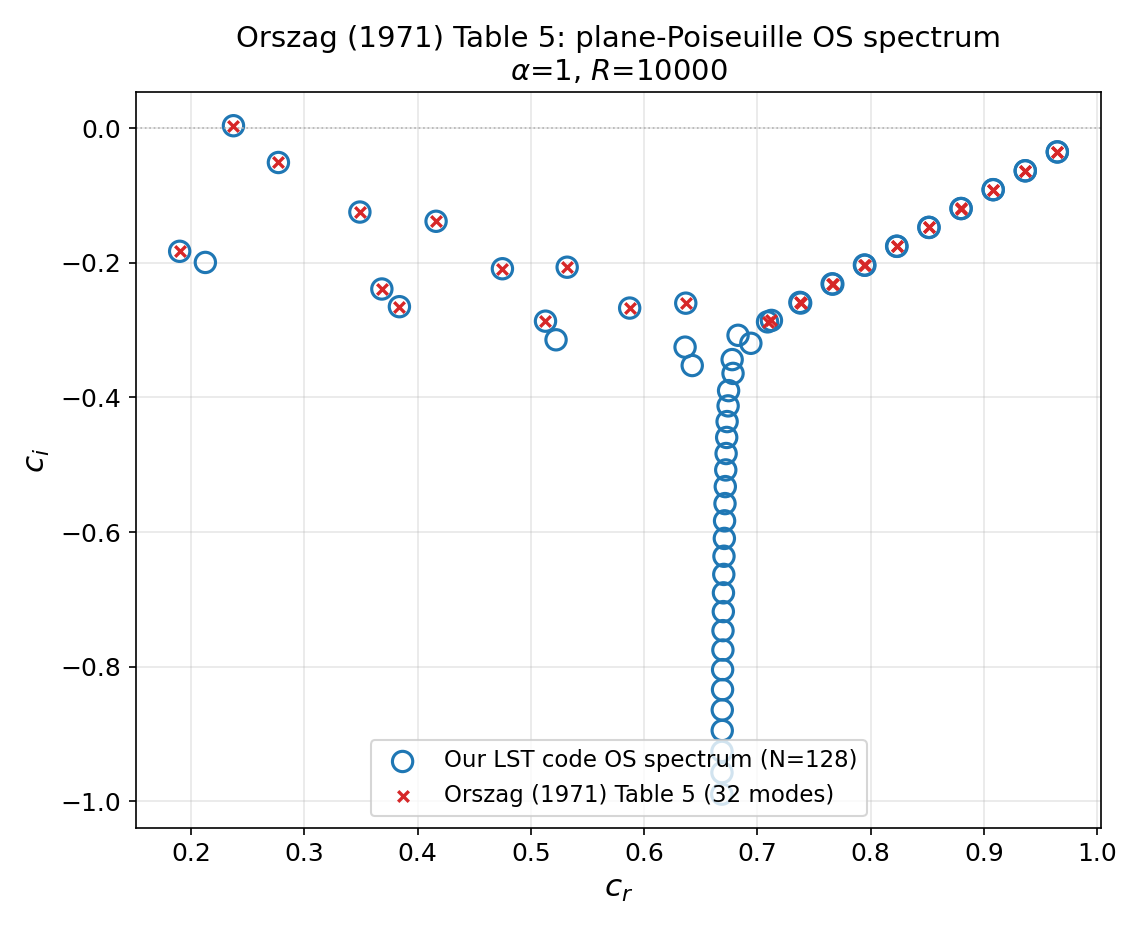
\includegraphics[width=0.72\linewidth]{../verification/other/orszag_spectrum/overlay.png}
\caption{Orszag Table~5 \cite{orszag1971}: Our LST code's plane-Poiseuille Orr--Sommerfeld
spectrum (circles) over the 32 tabulated eigenvalues (crosses), $\alpha=1$, $R=10\,000$. The
classic ``Y''-shaped spectrum (A-, P-, and S-branches), with every tabulated mode matched to
$<10^{-5}$.}
\label{fig:orszag-spectrum}
\end{figure}

\FloatBarrier
%=====================================================================
\section{Compressible eigenvalue anchors}
\label{sec:anchors}
%=====================================================================

\subsection{Malik (1990): compressible eigenvalue anchors}
\label{sec:malik}

\paragraph{Reference.} Malik \cite{malik1990}, the standard tabulated compressible-LST
test-case suite. Case~6 (Table~IX, the $M=4.5$ spatial second mode) is the primary anchor,
cross-checked digit-for-digit against Xi, Ren \& Fu \cite{xirenfu2020} and Hildebrand et al.\
\cite{hildebrand2018}. Cases 3, 4, 5 (Tables~IV/V/VI) and the grid-refinement case of Table~X were
long non-reproducible for want of their dimensional conditions (\cite{hildebrand2018} lists only $M$
and $R$), until Malik's own Table~I supplied the missing $T_0$ and wall temperatures, in particular
case~4's \emph{cooled} wall $T_w/T_{\rm adb}=0.1$ that earlier attempts had assumed adiabatic.

\paragraph{Conditions.} All cases share $Pr=0.7$, $\gamma=1.4$, Sutherland $S=110.33$~K, $L^\ast$
length scale. The suite spans $M=2.5$--$10$, temporal (fixed real $\alpha$, complex $\omega$) and
spatial (fixed real $\omega$, complex $\alpha$) formulations, and adiabatic and cooled walls.
Case~3 ($M=2.5$, oblique $\beta=0.1$) is a first mode; the rest are second (Mack) modes.
Each anchor is Chebyshev-collocated at $N=120$--$280$ points (larger $N$ for the thick $M=10$
layers), domain height $y_{\max}=40$--$140\,\delta^\ast/L^\ast$, $L^\ast$ scaling, with an isothermal
disturbance-temperature condition and bulk-viscosity ratio $\lambda/\mu=1.2$.

Both formulations of the collocation route appear, matched case by case to what Malik tabulates:
the temporal cases 3--5 use the temporal GEVP (its 3-D variant for the oblique case 3), returning
the complex frequency $\omega$ from a real wavenumber, while the spatial cases 6 and Table~X use the
spatial quadratic eigenvalue problem in companion form with shift--invert targeting, returning the
complex wavenumber $\alpha$ from a real frequency. Table~\ref{tab:malik} lists the five anchors. Every real part ($\alpha_r$ or $\omega_r$) is
essentially exact, fixing each mode and its phase speed. The one outlier is Table~X's \emph{spatial}
$\alpha_i$, which reflects the documented hypersonic-second-mode inter-method spread: Tumin's
recomputation of case~6's $\alpha_i$ from Malik's printed value differs in the same way, and the
solver of \cite{xirenfu2020} gives $-0.002780$. The \emph{temporal} $M=10$ growth rates (cases 4,
5) match closely, so the spatial $\alpha_i$ is the more formulation-sensitive quantity. Case~5 is
Malik's deliberately near-neutral ``severe test'': his own SDSP scheme flips $\omega_i$ negative at
coarse resolution, yet Our LST code lands on his converged value (Figure~\ref{fig:malik5}).

\begin{table}[htbp]
\centering\small
\caption{The Malik \cite{malik1990} compressible eigenvalue anchors. Spatial cases (6, X) compare
the complex wavenumber $\alpha$; temporal cases (3--5) compare the complex frequency $\omega$.}
\label{tab:malik}
\begin{tabular}{@{}p{1.7cm}p{3.9cm}p{3.6cm}p{3.6cm}@{}}
\toprule
Case & Conditions & Our LST code & Malik \\
\midrule
6 (Tab.~IX) & $M4.5$ adiab., spatial 2nd & $0.253400{-}0.002490\,\imag$ & $0.253405{-}0.002492\,\imag$ \\
3 (Tab.~IV) & $M2.5$ oblique, temporal 1st & $0.036735{+}0.000584\,\imag$ & $0.036734{+}0.000584\,\imag$ \\
4 (Tab.~V) & $M10$ cooled, temporal 2nd & $0.097457{+}0.001988\,\imag$ & $0.097484{+}0.002030\,\imag$ \\
5 (Tab.~VI) & $M10$ adiab., temporal 2nd & $0.115862{+}0.000156\,\imag$ & $0.115865{+}0.000153\,\imag$ \\
X (Tab.~X) & $M10$ cooled, spatial 2nd & $0.095803{-}0.002403\,\imag$ & $0.095933{-}0.002156\,\imag$ \\
\bottomrule
\end{tabular}
\end{table}

\begin{figure}[H]
\centering
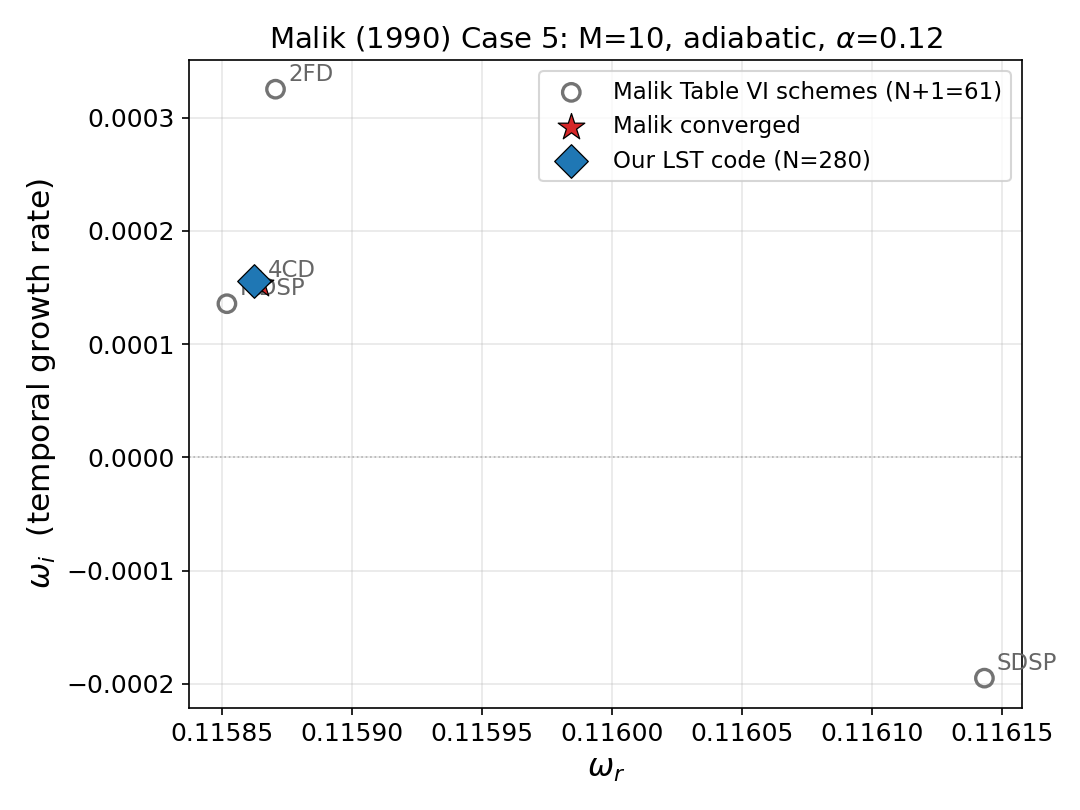
\includegraphics[width=0.72\linewidth]{../verification/second_mode/malik_case5/overlay.png}
\caption{Malik case~5 \cite{malik1990} ($M=10$ adiabatic, the deliberately near-neutral ``severe
test''): Our LST code (diamond) lands on Malik's converged value (star) and his 4CD/MDSP
cluster, while his own 2FD scheme sits high and SDSP flips $\omega_i$ negative;
Our LST code reproduces the case Malik built to break solvers.}
\label{fig:malik5}
\end{figure}

\subsection{Malik (1990) Fig.~4: M10 second-mode eigenfunction}
\label{sec:malik-fig4}

\paragraph{Reference.} Malik \cite{malik1990}, Fig.~4: the disturbance eigenfunctions of the same
$M=10$ cooled-wall condition as case~4. The comparison uses the temperature eigenfunction
$\hat T$ (real and imaginary parts), the dominant, cleanly traceable curves; the small velocity
and pressure eigenfunctions overlap near the axis and are not reliably digitisable, so they are
omitted.

At the case-4 conditions ($N=200$ Chebyshev points, $y_{\max}=75\,\delta^\ast/L^\ast$, $L^\ast$
scaling, isothermal disturbance-temperature condition) the temporal GEVP is read for its
eigen\emph{vector} rather than its eigenvalue: from a real wavenumber $\alpha$ it returns the
discrete eigenpair, of which the temperature component $\hat T(y)$ is compared. This is therefore a mode-shape check, not an
eigenvalue one, and the complex temperature eigenfunction $\hat T(y)$ is normalised so that
$\hat T_r$ peaks at $+1$ (Malik's convention, which fixes the eigenvector's single global phase).
Both the real and imaginary temperature eigenfunctions lie on the digitised Fig.~4 points
(Figure~\ref{fig:malik-fig4}). Our LST code's $\hat T_r$ traces the near-wall negative lobe, the
zero crossing near $y\!\approx\!6$, and the sharp unit peak at $y=13.3$ ($\approx\delta^\ast$)
against Malik's $\approx13$; $\hat T_i$ reproduces the same double-lobed shape, a positive hump
near $y\!\approx\!11$ and a negative dip near $y\!\approx\!15$. Under the \emph{single} global phase
that makes $\hat T_r$ real at its peak, \emph{both} parts fall on the reference, so the temperature
eigenvector is validated in full, not merely its peak location. The temperature fluctuation
dominates the velocity ($|\hat T|/|\hat u|\approx14$), the hallmark of the hypersonic Mack mode.

\begin{figure}[H]
\centering
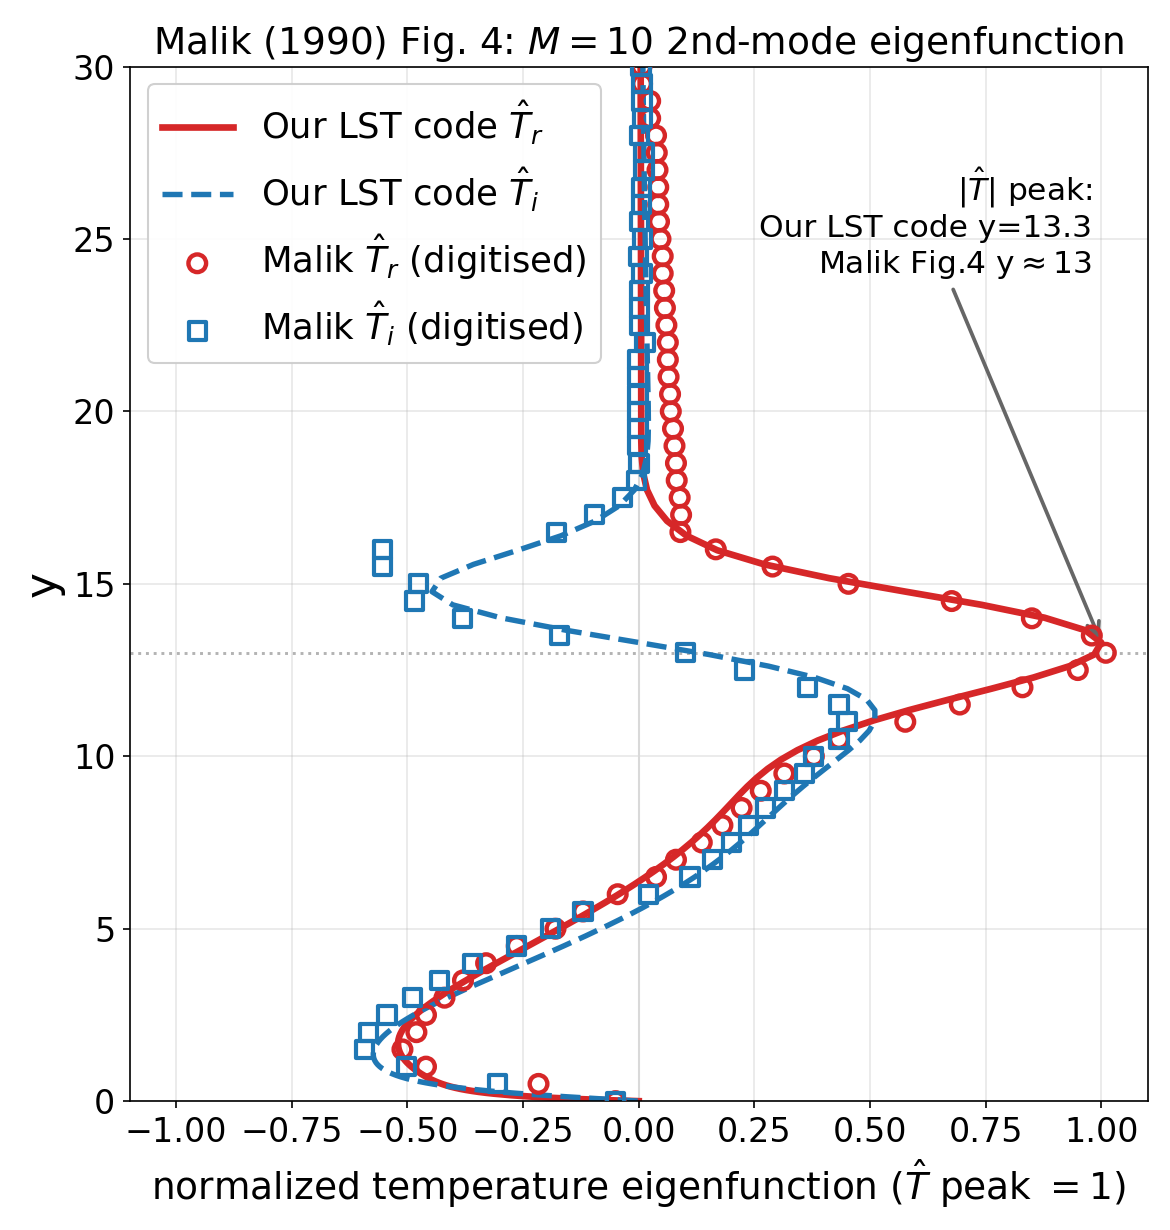
\includegraphics[width=0.72\linewidth]{../verification/second_mode/malik_fig4_eigenfunction/overlay.png}
\caption{Malik Fig.~4 \cite{malik1990}, $M=10$ second-mode temperature eigenfunction: Our LST
code's $\hat T_r$ (solid) and $\hat T_i$ (dashed) curves over the digitised points, normalised so
$\hat T_r$ peaks at $+1$. Both parts match under a single global phase: $\hat T_r$ has its unit peak
at $y=13.3$ against Malik's $\approx13$, and $\hat T_i$ shows the positive hump near
$y\!\approx\!11$ and the negative dip near $y\!\approx\!15$.}
\label{fig:malik-fig4}
\end{figure}

\subsection{Balakumar \& Malik (1992): discrete/continuous spectrum topology}
\label{sec:bm1992}

\paragraph{Reference.} Balakumar \& Malik \cite{balakumar1992}. The paper presents its branches
graphically; no tabulated branch eigenvalues are openly recoverable, so this is a qualitative
branch-topology check plus a fully specified spatial second-mode cross-check.

\paragraph{Conditions.} $M=4.5$, $T_0=311$~K, $Re=1000$, $\omega=0.2$, adiabatic (insulated) wall.
The full companion spectrum is computed by Chebyshev collocation at $N=120$ ($121$ nodes),
$y_{\max}=40\,\delta^\ast/L^\ast$, $L^\ast$ scaling, with an isothermal disturbance-temperature
condition and $\lambda/\mu=1.2$.

The spatial quadratic eigenvalue problem is solved for its \emph{entire} companion spectrum, not
merely the shift--invert neighbourhood: from a real frequency $\omega$ it returns all complex
wavenumbers $\alpha$ of the discretised operator at once, discrete mode and rendered continuous
spectrum together, which is what a branch-topology comparison requires. The comparison is thus
twofold: the branch topology (how the discrete second mode separates from the continuous spectrum in
the complex-$\alpha$ plane) and the discrete spatial eigenvalue $\alpha$. Our LST code's full
spatial spectrum reproduces the published topology: the discrete second mode
sits at $\alpha=0.220210-0.002787\,\imag$ ($c=0.9082$), matching the published
$0.220-0.003091\,\imag$, and is the unique least-damped root in the second-mode phase-speed band,
while a cluster of roots accumulates at the freestream phase speed $c\!\to\!1$ (the continuous
spectrum). The discrete mode is set apart from that cluster in phase speed and growth rate, not by a
wide gap in the complex plane: the discretised continuum is dense in $\alpha_r$, so the nearest
continuum root lies close by, the expected signature of the continuous spectrum crowding the
discrete mode. Treated purely as a spatial second-mode anchor, the real part is essentially exact and
the imaginary part carries the same inter-method $\alpha_i$ spread seen on Malik case~6
(Figure~\ref{fig:bm1992}).

\begin{figure}[H]
\centering
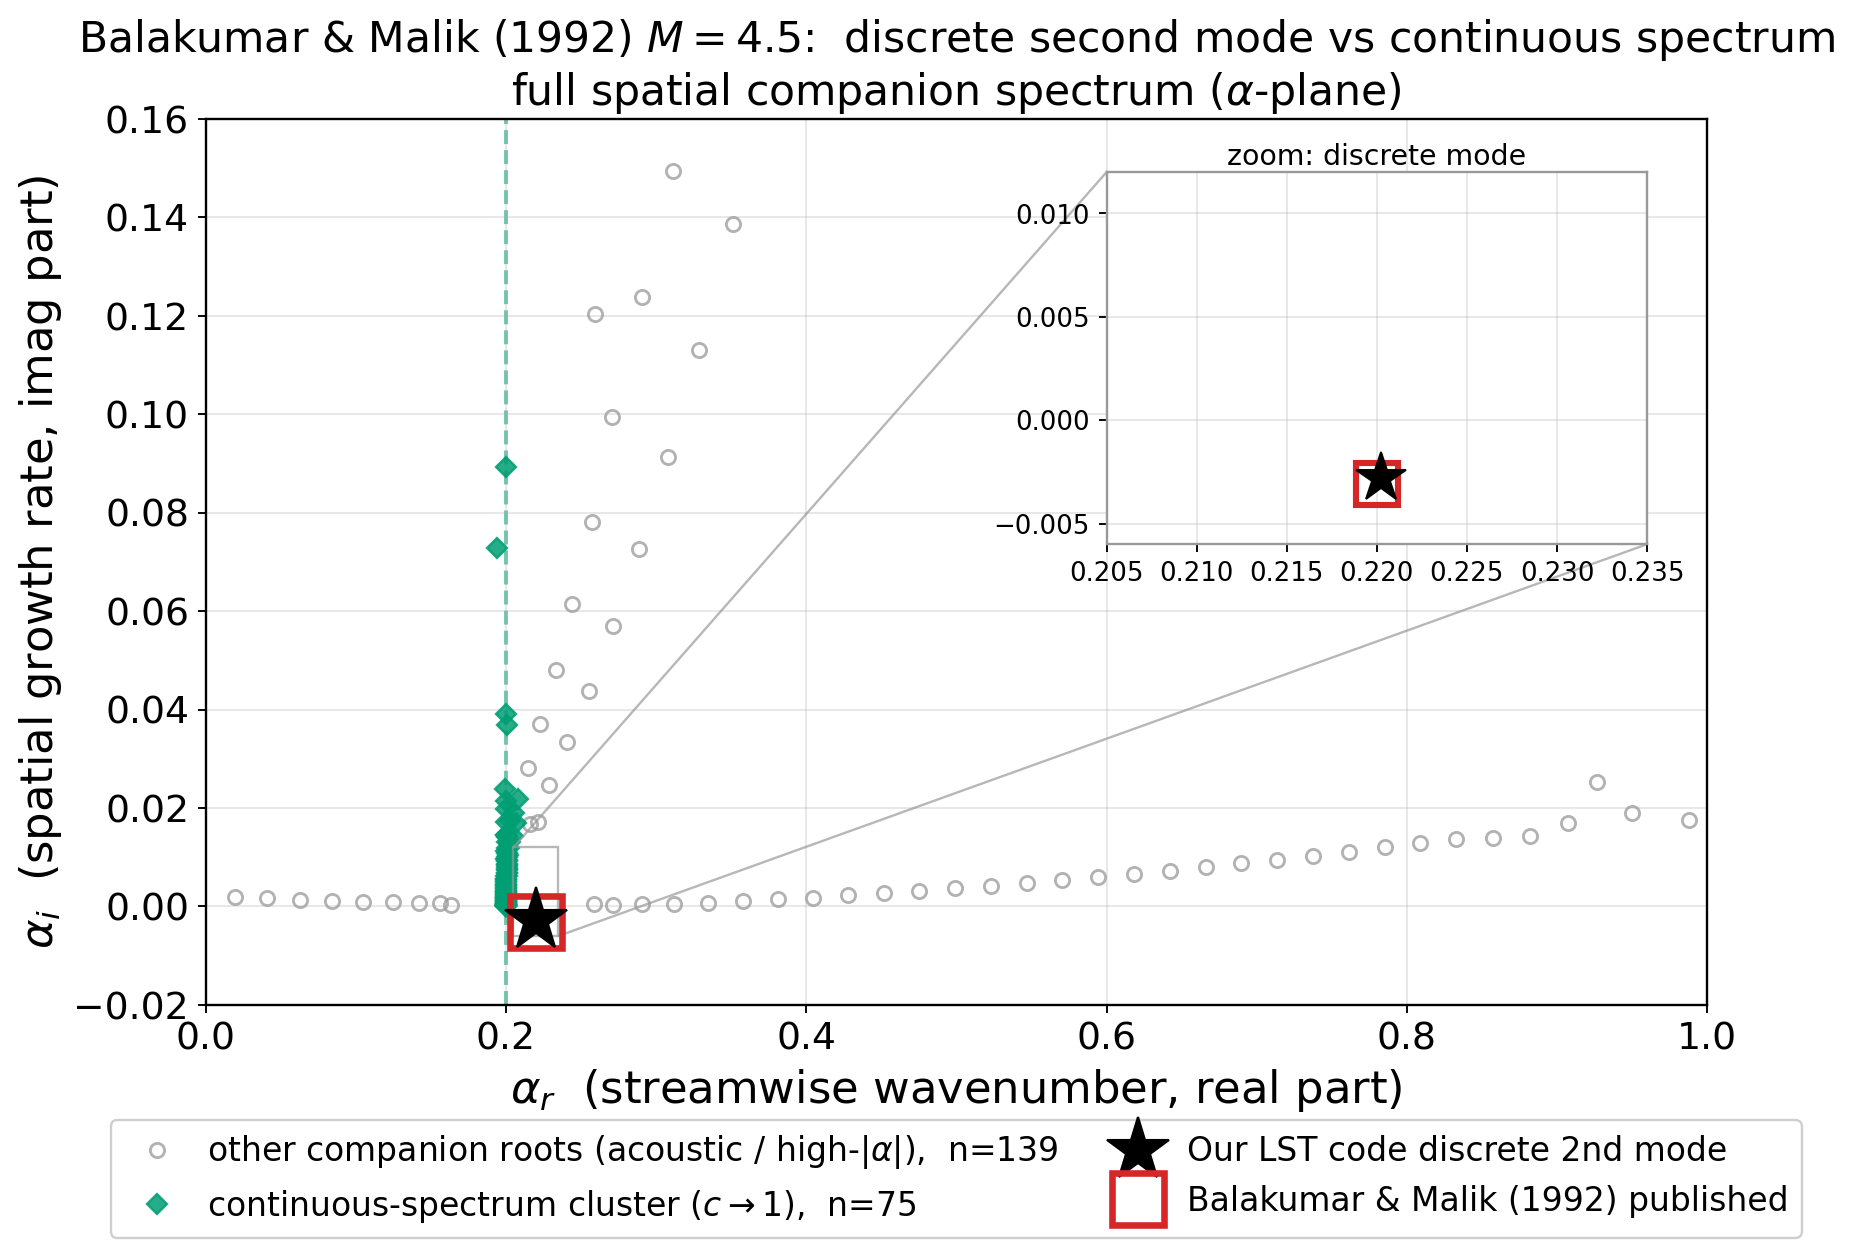
\includegraphics[width=0.75\linewidth]{../verification/second_mode/balakumar_malik1992_branches/overlay.png}
\caption{Balakumar \& Malik \cite{balakumar1992}, $M=4.5$: Our LST code's complex-$\alpha$
spectrum showing the discrete second mode set apart (in phase speed and growth rate) from the
continuous-spectrum cluster near $c\!\to\!1$.}
\label{fig:bm1992}
\end{figure}

\FloatBarrier
%=====================================================================
\section{Second mode: curves and families}
\label{sec:secondmode}
%=====================================================================
Having pinned the compressible operator at single points, the following cases test full
growth-rate and neutral curves; the second mode is Our LST code's design target.

\subsection{Mack (1984) Fig.~10.6: second-mode growth vs.\ Reynolds number}
\label{sec:mack106}

\paragraph{Reference.} Mack \cite{mack1984}, Fig.~10.6.

\paragraph{Conditions.} Air, adiabatic wall, 2-D wave ($\psi=0^\circ$), at $M=4.5$, $5.8$, $7$, and
$10$. Two modelling choices make the comparison defensible: the cold edge state of Mack's
Table~11.1 \cite{mack1984} (resolving a historical $\sim\!6\times$ gap that was an
edge-temperature error) and a
wall-normal domain $y_{\max}\approx4\,\delta^\ast/L^\ast$ that grows with Mach ($y_{\max}=40$ at
M4.5 up to $140$ at M10; a fixed short box starves the thick high-Mach boundary layer). The
eigenvalue solves use Chebyshev collocation at $N=110$, $L^\ast$ scaling, and the 2-D Stokes
closure $\lambda/\mu=0$.

Sweeping the temporal GEVP in wavenumber at each Reynolds number (a real $\alpha$ scan at fixed $R$,
from which the second-mode $\omega_i=\alpha c_i$ is maximised over $\alpha$, then repeated over $R$)
traces the curve. Across $M=4.5$, $5.8$, $7$, and $10$, Our LST code's maximum second-mode temporal
growth rate $\omega_{i,\max}(R)$ (Mack's $L^\ast$ scale, $c_r\approx0.9$) tracks the digitised
Fig.~10.6 points. The match is tightest at $M=7$ and $M=10$ and carries a small residual at $M=4.5$
and $M=5.8$; because both ends of the Mach range match well, that residual is local rather than a
monotonic high-Mach under-prediction. The $M=4.5$ and $M=10$ curves are shown as representatives
(Figures~\ref{fig:mack106_m45} and \ref{fig:mack106_m100}); $M=5.8$ and $M=7$ follow the same trend
and are summarised in Table~\ref{tab:summary}.

\begin{figure}[H]
\centering
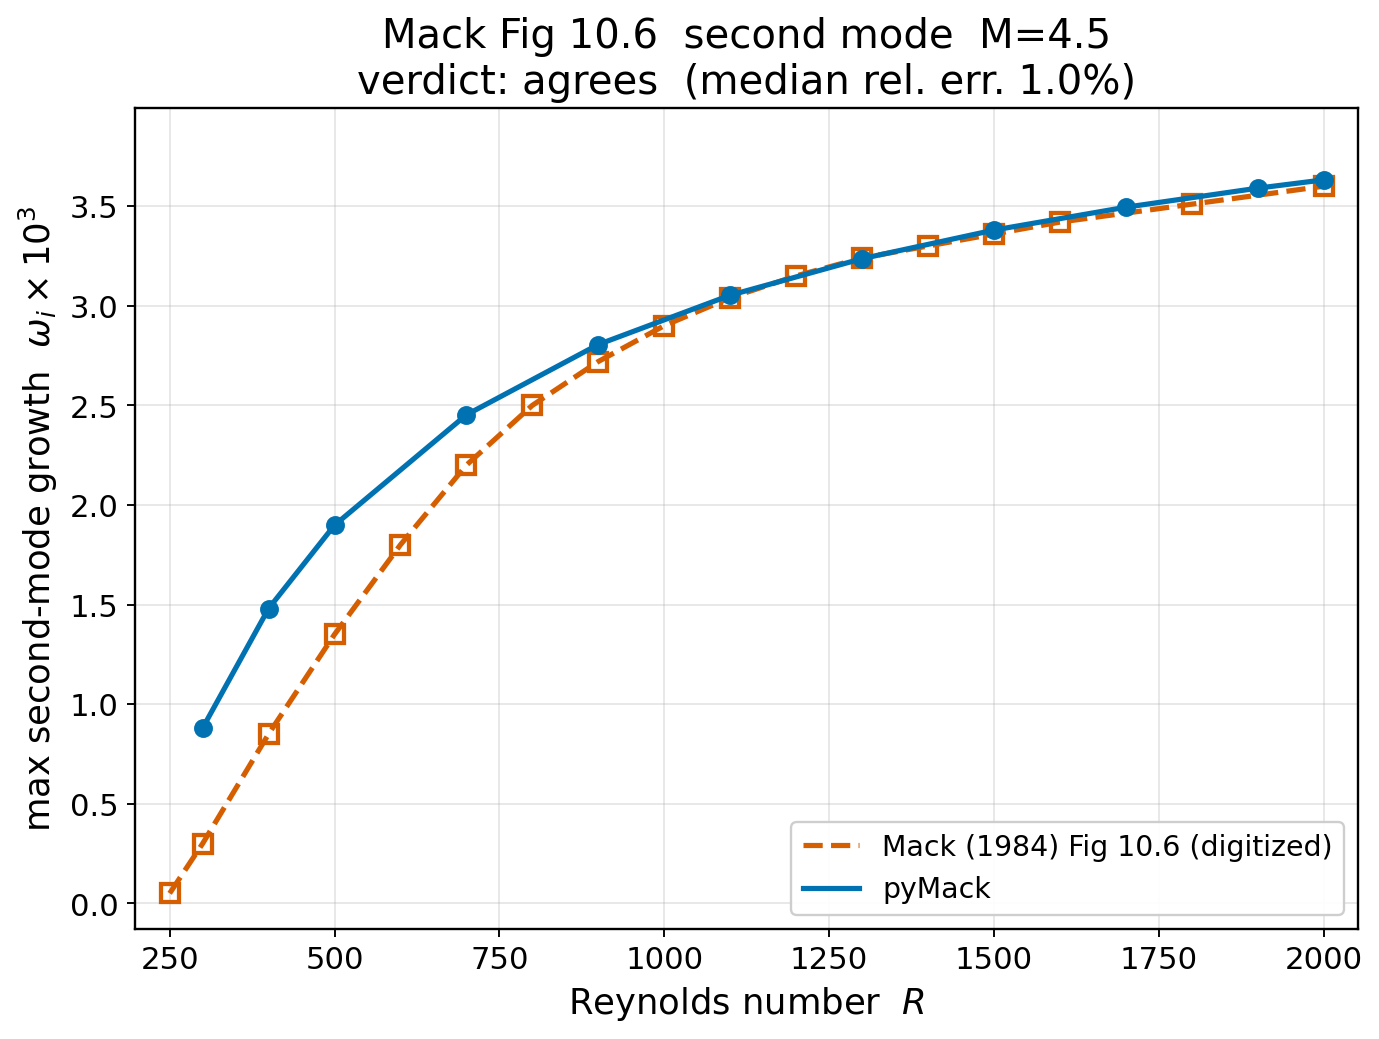
\includegraphics[width=0.75\linewidth]{../verification/second_mode/mack_fig10_6_M45/overlay.png}
\caption{Mack Fig.~10.6 \cite{mack1984}, $M=4.5$: Our LST code's $\omega_{i,\max}(R)$ over the
digitised points, with a small residual at this Mach number.}
\label{fig:mack106_m45}
\end{figure}

\begin{figure}[H]
\centering
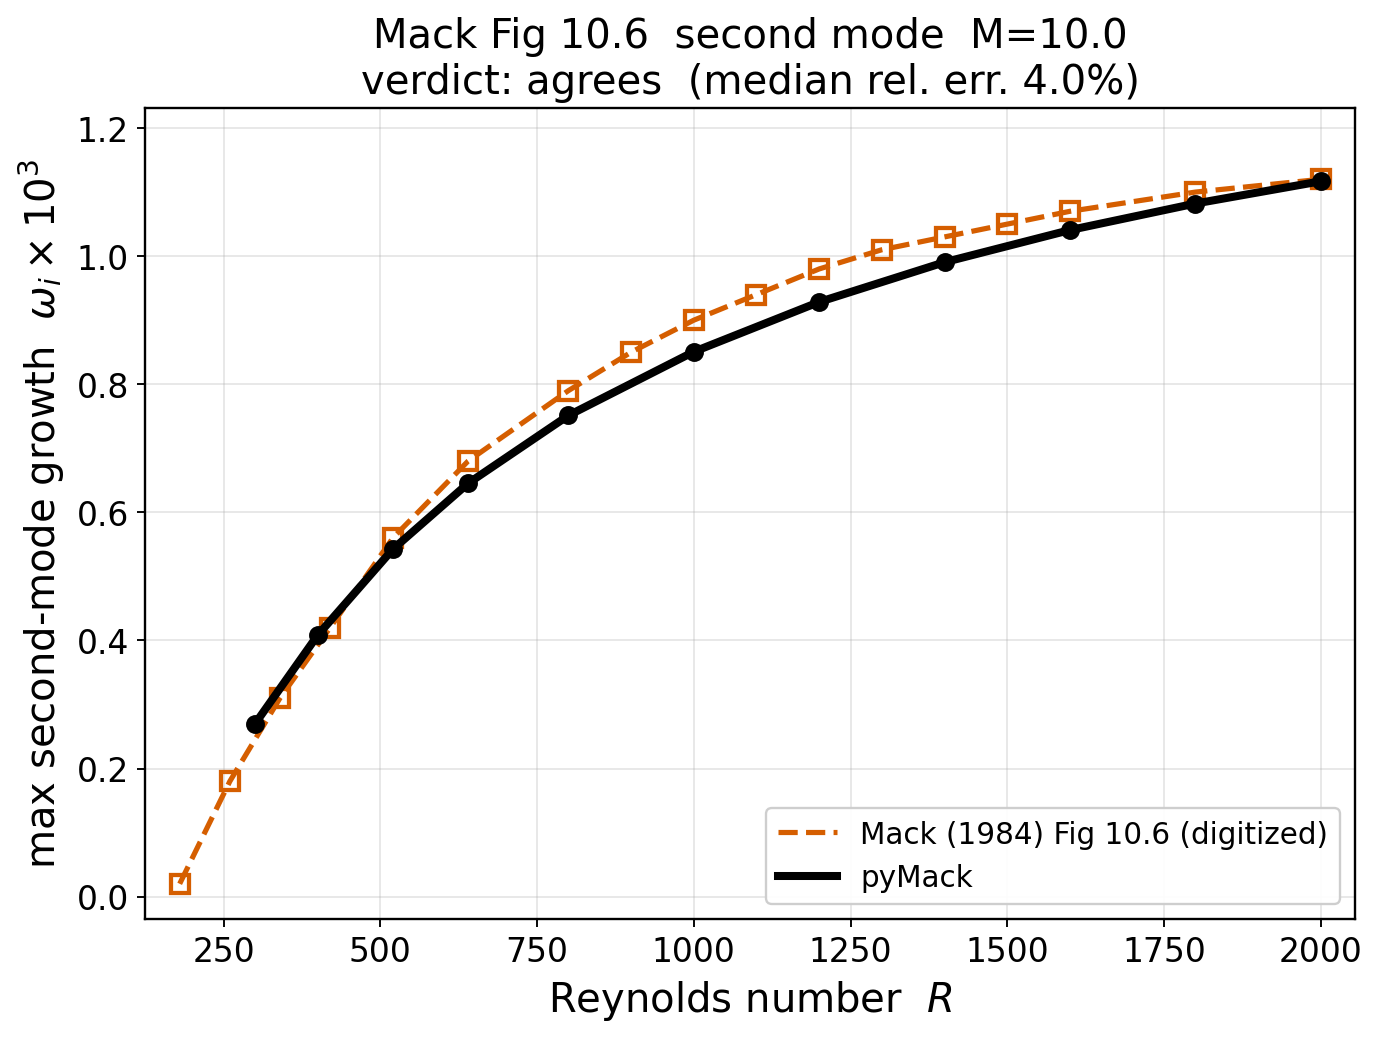
\includegraphics[width=0.75\linewidth]{../verification/second_mode/mack_fig10_6_M100/overlay.png}
\caption{Mack Fig.~10.6 \cite{mack1984}, $M=10$: the same comparison at the top of the Mach range,
with the domain-converged ($y_{\max}=140$), cold-edge second mode.}
\label{fig:mack106_m100}
\end{figure}

\subsection{Egorov et al.\ (2006): Mach-6 flat-plate second mode}
\label{sec:egorov}

\paragraph{Reference.} Egorov, Fedorov \& Soudakov \cite{egorov2006}: 2-D DNS second-mode growth
over a Mach-6 adiabatic flat plate, reported to agree with LST.

\paragraph{Conditions.} Perfect gas $\gamma=1.4$, $Pr=0.72$, power-law viscosity
$\mu/\mu_e=(T/T_e)^{0.7}$; $M_\infty=6$, $Re_L=2\times10^6$, adiabatic wall; mode-S circular
frequency $\omega\approx200$ (plate-length units) at the synchronisation location $x=1$
($R=\sqrt{2\times10^6}=1414$). The spatial solve uses Chebyshev collocation at $N=140$,
$y_{\max}=40\,\delta^\ast/L^\ast$, $L^\ast$ scaling, an isothermal disturbance-temperature
condition, and $\lambda/\mu=1.2$.

The spatial QEP is swept in frequency at the synchronisation location $R=1414$ (real $\omega$ across
the candidate band, returning the complex wavenumber $\alpha$ and hence the spatial growth
$\sigma=-\alpha_i$ and its maximiser). Because the paper presents the DNS-vs-LST comparison as a
growth-rate-vs-$x$ curve with no printed growth-rate digit, the comparison is made on the
second-mode instability band and the frequency of the most-amplified mode. Our LST code's discrete second mode ($c_r\approx0.92$--$0.94$) is unstable
across
$\omega_E\in[140,260]$, which brackets the reference forcing $\omega=200$, and is most-amplified at
$\omega_E\approx215$; at exactly $\omega=200$ the spatial growth is $-\alpha_i=2.90\times10^{-3}$
with $c_r=0.934$. Our LST code thus places the M6 second-mode instability squarely in the stated
band, with the most-amplified frequency essentially on the reference forcing choice.

\subsection{Ma \& Zhong (2003) Fig.~15: M4.5 second-mode neutral curve}
\label{sec:mazhong}

\paragraph{Reference.} Ma \& Zhong \cite{mazhong2003}, \S6 / Fig.~15: full neutral curves
$\omega(R)$ for the first and second mode at $M=4.5$, with the second-mode branch points quoted in
text at $R=806$ (branch~I) and $R=999.6$ (branch~II) for $F=2.2\times10^{-4}$.

\paragraph{Conditions.} Air, adiabatic \emph{mean} wall, 2-D ($\psi=0^\circ$), $M=4.5$,
$T_e=65.15$~K, unit $Re=7.2\times10^6$/m, Sutherland $S=110.33$~K, $Pr=0.72$, $\gamma=1.4$;
spatial formulation at fixed $F=2.2\times10^{-4}$. The \emph{disturbance} temperature wall
condition is isothermal ($\hat{T}|_{w}=0$), which the authors state they used for the Fig.~15
neutral curve. The spatial sweeps use Chebyshev collocation at $N=130$ ($131$ nodes),
$y_{\max}=40\,\delta^\ast/L^\ast$, $L^\ast$ scaling, and $\lambda/\mu=1.2$.

The spatial QEP is run in fixed-frequency sweeps: real $\omega$ along each $F=\mathrm{const}$ path
in $R$ returns the complex wavenumber, and the neutral curve is the $\sigma=-\alpha_i=0$ crossing
set; the first-mode branches use the same route with the discrete-mode selector (freestream decay
$+$ $y_{\max}$-stationarity). Our LST code thus traces the full neutral curve $\omega(R)$, anchored
against the two second-mode branch points quoted in the text at $F=2.2\times10^{-4}$. Its
second-mode neutral band reproduces the closed loop of Fig.~15 (nose near $R\approx280$, upper
branch $\omega\approx0.225$, lower branch $\omega\approx0.18$) across the full range. At the quoted $F=2.2\times10^{-4}$, the band crosses at $R=786.6$ (branch~I; text value
$806$) and $R=1009.9$ (branch~II; text value $999.6$). Using the adiabatic disturbance condition by
mistake shifts these to $831$ and $1033$; the paper's actual isothermal disturbance condition is a
correction, not a fit, and tightens the match. The first-mode \emph{cutoff} (upper) branch,
re-extracted with the discrete-mode selector (freestream decay $+$ $y_{\max}$-stationarity,
replacing the earlier phase-speed-band classifier), follows Fig.~15's upper branch closely. The
low-$\omega$ \emph{onset} (lower) branch is \emph{not} recovered: below $\omega\approx0.03$ the 2-D
first mode ($c_r\!\lesssim\!0.45$) delocalises into the slow-acoustic continuous spectrum
($c_r\le1-1/M=0.778$), leaving no clean discrete eigenmode. This limit is the same across Our LST
code's spatial and temporal collocation solvers and a QR-shooting variant, and a wave-angle sweep
confirms the 2-D mode is the most unstable here (so this is a 2-D, not an oblique, first mode).
Recovering the onset branch would need a compound-matrix shooting solver robust to the
near-continuous-spectrum decay rates, which is left as an open item in the companion working note
(Figure~\ref{fig:mazhong}).

\begin{figure}[H]
\centering
\includegraphics[width=0.85\linewidth]{../verification/second_mode/mazhong2003_m4p5/overlay_fig15_full.png}
\caption{Ma \& Zhong Fig.~15 \cite{mazhong2003}, $M=4.5$: Our LST code's second-mode neutral loop
over the pixel-digitised Fig.~15 points, matching the branch points at $F=2.2\times10^{-4}$
($R=786.6$ vs.\ $806$; $R=1009.9$ vs.\ $999.6$) under the isothermal disturbance condition. The
first-mode \emph{cutoff} branch, re-extracted with the discrete-mode selector, follows the
digitised upper branch; the first-mode \emph{onset} (shaded band) is continuous-spectrum-limited,
the long-wavelength mode delocalising into the continuous spectrum, a limit shared by all of Our
LST code's collocation and QR-shooting methods (see text).}
\label{fig:mazhong}
\end{figure}

\FloatBarrier
%=====================================================================
\section{First mode: curves and families}
\label{sec:firstmode}
%=====================================================================
The first mode was Our LST code's documented weak spot. After a reference-digitisation
correction, most of the Mack first-mode figures now match well; the remaining disagreement is
narrow and isolated to the $M\approx2.2$ cases (Fig.~10.1 and Fig.~10.3 at $M=2.2$), a genuine
under-amplification and too-high critical Reynolds number at that Mach rather than a general trend,
and is tracked in the companion working note. This section reports the Mack first-mode figures;
the \"Ozgen--K{\i}rcal{\i} neutral-curve family, whose figures carry first-mode branches alongside
second-mode ones, is treated separately in Section~\ref{sec:mixedmode}.

\subsection{Mack (1984) Fig.~10.1: first-mode neutral loop}
\label{sec:mack101}

\paragraph{Reference.} Mack \cite{mack1984}, Fig.~10.1, the innermost (complete-equations) neutral
loop, re-digitised with both branches plus nose.

\paragraph{Conditions.} Air, adiabatic wall, 2-D ($\psi=0^\circ$), at $M=1.6$ and $M=2.2$;
temporal neutral loop ($c_i=0$) in $(R, F\!\times\!10^4)$. The $(R,\alpha)$-grid solves use Chebyshev
collocation at $N=140$, $y_{\max}=45\,\delta^\ast/L^\ast$, $L^\ast$ scaling, and $\lambda/\mu=0$.

Solving the temporal GEVP over an $(R,\alpha)$ grid (real $\alpha$ at each $R$, returning the
complex phase speed) gives the neutral loop as the $c_i=0$ contour, with the critical Reynolds
number at its nose. At $M=1.6$ the first-mode neutral loop (its lower onset and upper cutoff
branches) closely tracks Mack's complete-equations loop after the corrected reference, with critical
Reynolds number $R\approx300$ against Mack's $\approx215$
(Figure~\ref{fig:mack101_m16}). The companion $M=2.2$ loop shows a genuine first-mode
under-amplification, with a too-high critical Reynolds number ($R\approx400$ against Mack's
$\approx300$), and is documented in the companion working note.

\begin{figure}[H]
\centering
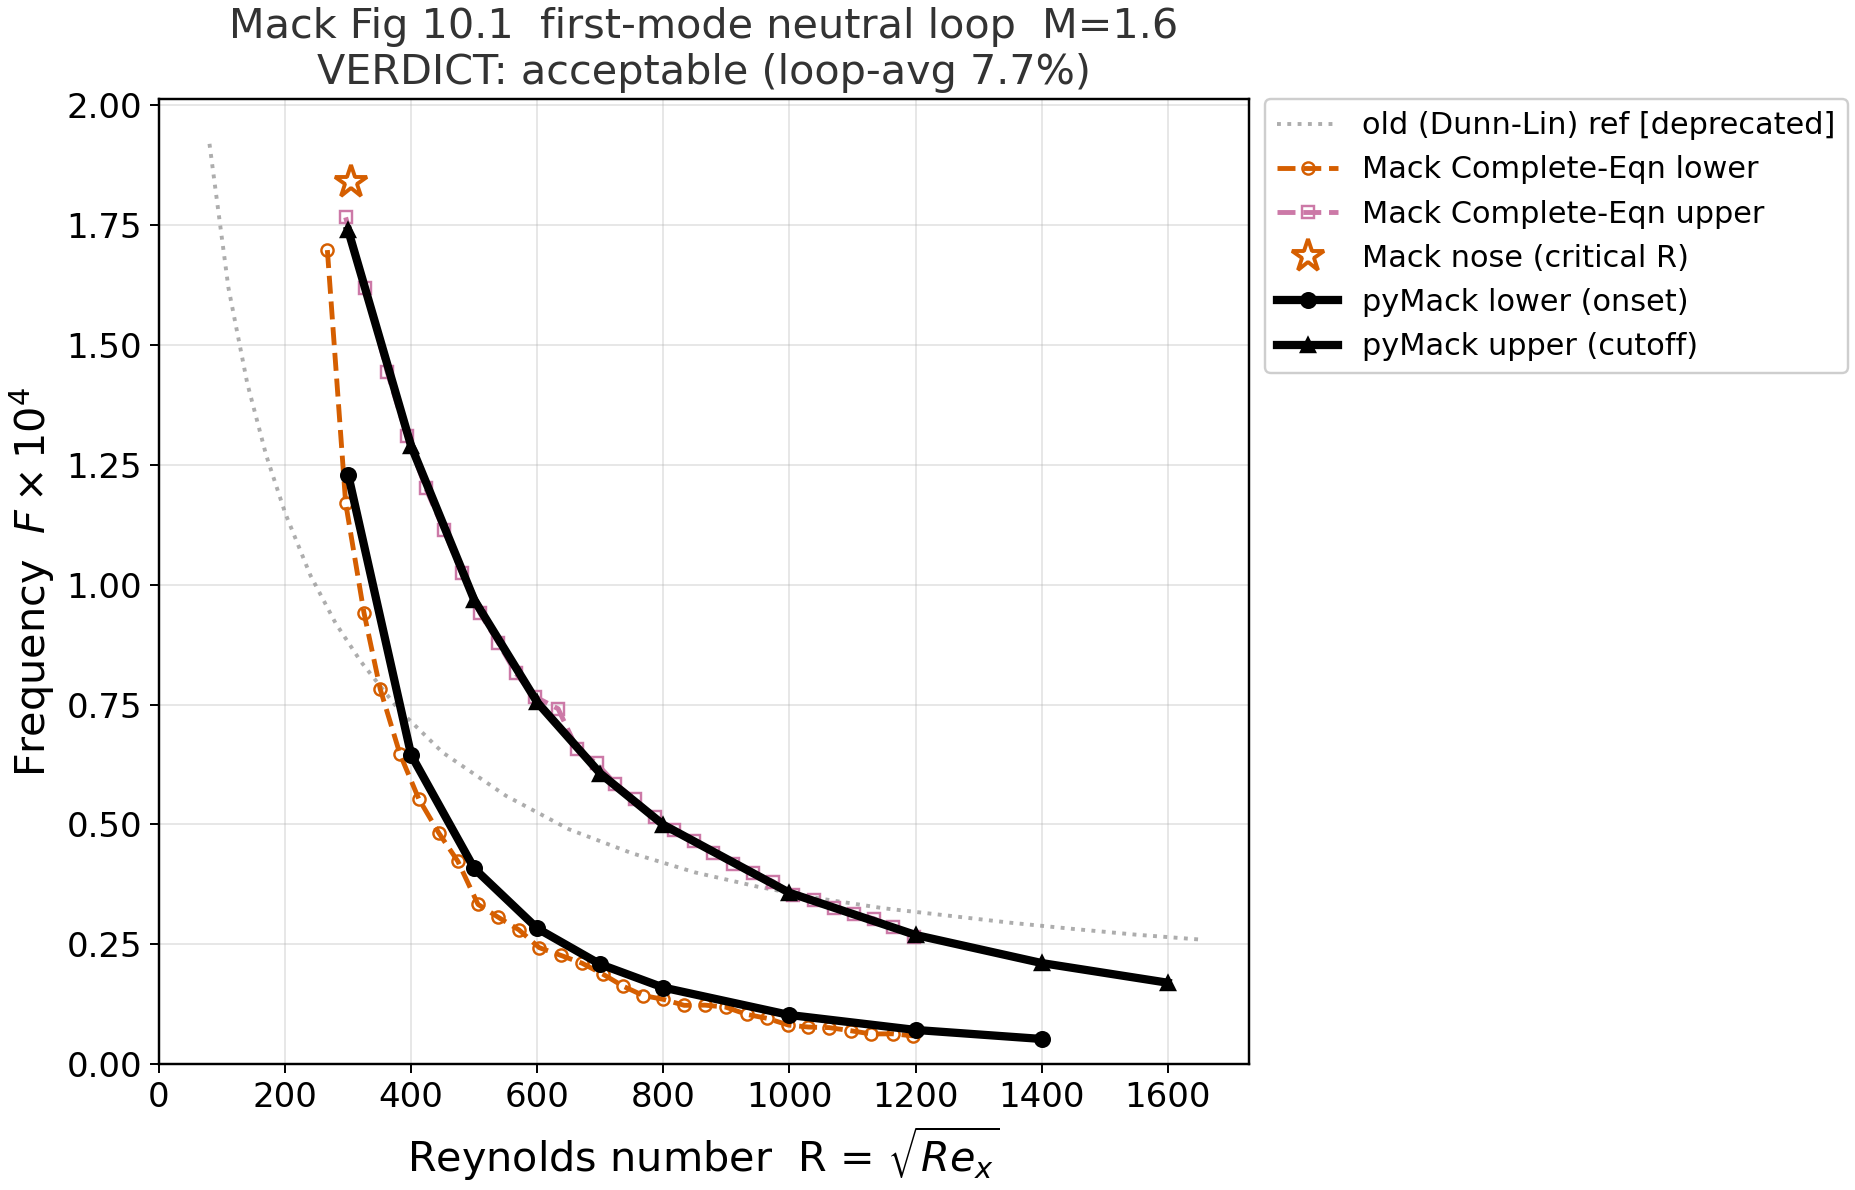
\includegraphics[width=0.75\linewidth]{../verification/first_mode/mack_fig10_1_m1p6/overlay.png}
\caption{Mack Fig.~10.1 \cite{mack1984}, $M=1.6$: Our LST code's first-mode neutral loop closely
tracks Mack's complete-equations loop, with critical Reynolds number $R\approx300$ against Mack's
$\approx215$.}
\label{fig:mack101_m16}
\end{figure}

\subsection{Mack (1984) Fig.~10.3: oblique first-mode growth vs.\ $R$}
\label{sec:mack103}

\paragraph{Reference.} Mack \cite{mack1984}, Fig.~10.3.

\paragraph{Conditions.} Air (ideal, $Pr=0.72$), adiabatic wall; oblique waves at $M=1.3$
($\psi=45^\circ$), $M=2.2$ ($\psi=45^\circ$), $M=3.0$ ($\psi=60^\circ$). These oblique cases use the
exact $8\times8$ shooting march rather than a Chebyshev grid, with $y_{\max}\approx4\,\delta^\ast/L^\ast$
and $L^\ast$ scaling.

These curves use the exact oblique first-order \emph{shooting} route rather than the collocation
GEVP: at these Mach numbers the reduced temporal EVP's branch selection is not trusted, so an anchor
root is located by the $\sigma_{\min}(c)\to0$ search and continued in the parameters, with the
growth maximised over wavenumber at each $R$. At $M=1.3$ Our LST code's maximum first-mode temporal
growth $\omega_{i,\max}(R)$ tracks Fig.~10.3 closely and reproduces the rigorous Table-10.1
eighth-order anchor; $M=3.0$ tracks it as well. $M=2.2$ is the exception, a genuine
under-amplification (convergence-checked: not a $y_{\max}$ or step-count artifact). Topology is
correct in all three (a single rising-then-turning first-mode branch), so $M=2.2$ is an isolated
outlier rather than part of a growing-with-Mach trend. The $M=1.3$ case is shown in
Figure~\ref{fig:mack103_m13}; the $M=2.2$ case is documented in the companion working note.

\begin{figure}[H]
\centering
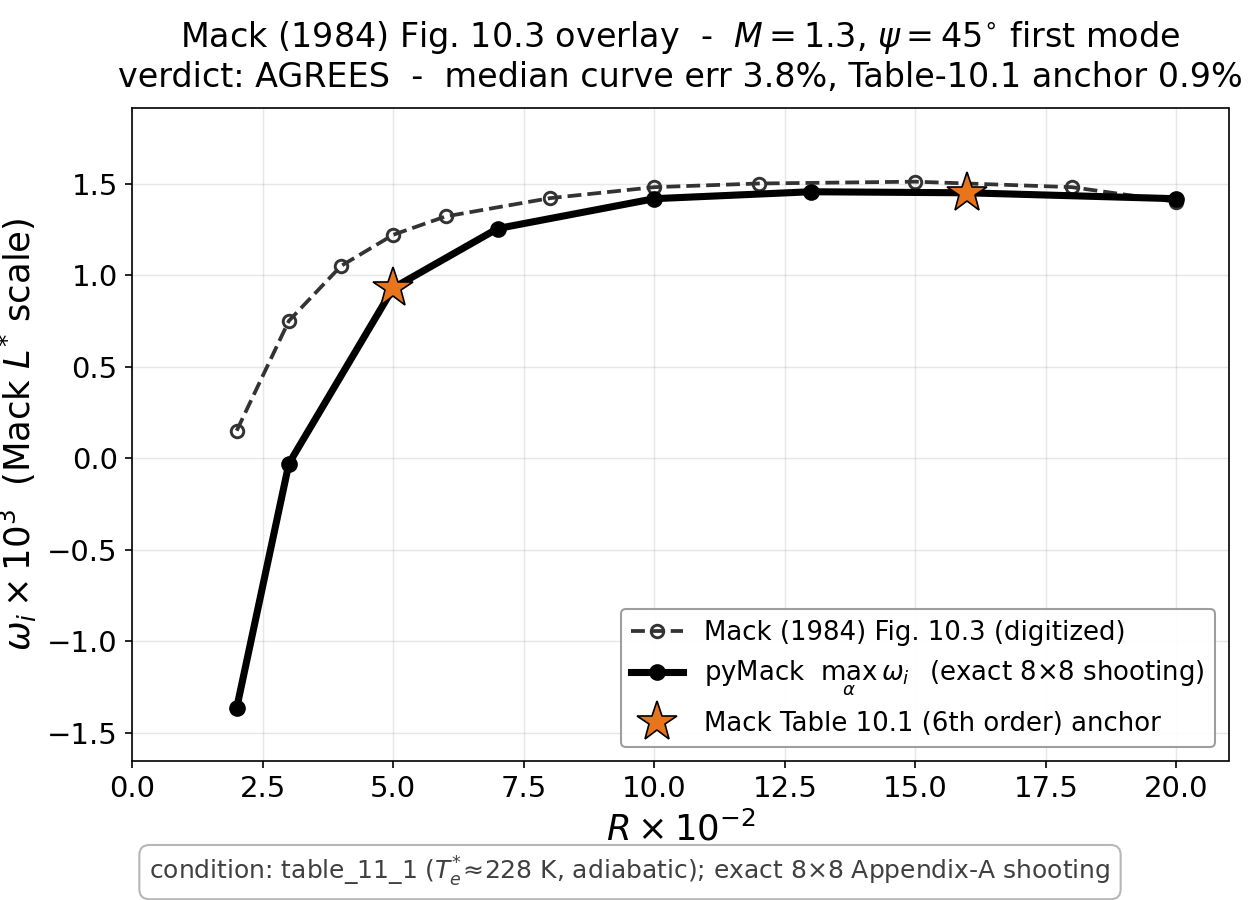
\includegraphics[width=0.75\linewidth]{../verification/first_mode/mack_fig10_3_m1p3/overlay.png}
\caption{Mack Fig.~10.3 \cite{mack1984}, $M=1.3$, $\psi=45^\circ$: Our LST code's
$\omega_{i,\max}(R)$ over the digitised points, reproducing the rigorous Table-10.1 eighth-order
anchor.}
\label{fig:mack103_m13}
\end{figure}

\subsection{Mack (1984) Fig.~10.4: oblique first mode at high Mach}
\label{sec:mack104}

\paragraph{Reference.} Mack \cite{mack1984}, Fig.~10.4.

\paragraph{Conditions.} Air, adiabatic wall; the high-Mach first mode is oblique-dominated, so
growth is maximised over both $\alpha$ and wave angle $\psi$; $M=4.5$, $5.8$, $7$, $10$ with
$y_{\max}\approx4\,\delta^\ast/L^\ast$. The 3-D temporal solves use Chebyshev collocation at $N=200$
($y_{\max}$ reaching $150\,\delta^\ast/L^\ast$ at $M=10$), $L^\ast$ scaling, and $\lambda/\mu=0$.

The reduced 3-D temporal GEVP takes the real oblique pair $\alpha$ and wave angle $\psi$
(equivalently $\beta$) and returns the complex frequency, with $\omega_i$ maximised over
$(\alpha,\psi)$ at each $R$. Across $M=4.5$, $5.8$, $7$, and $10$, Our LST code's maximum first-mode
temporal growth $\omega_{i,\max}(R)$ tracks the digitised Fig.~10.4 points, with the
oblique-first-mode peak near $\psi\approx60^\circ$ ($c_r\approx0.83$ at
$M=4.5$) and only a small residual at $M=10$, the top of the Mach range. One caveat: these curves
were computed with the reduced dense-EVP path rather than the exact-shooting path used for the
convergence-checked Fig.~10.3 cases, and no exact-shooting cross-check was recorded; the domain
used the second-mode-calibrated $\sim\!4\,\delta^\ast/L^\ast$ rule, while the first mode reaches
further from the wall. There is no first-mode under-amplification trend at high Mach in this figure.
$M=4.5$ and $M=10$ are shown (Figures~\ref{fig:mack104_m45} and \ref{fig:mack104_m100}); $M=5.8$ and
$M=7$ follow the same trend and are summarised in Table~\ref{tab:summary}.

\begin{figure}[H]
\centering
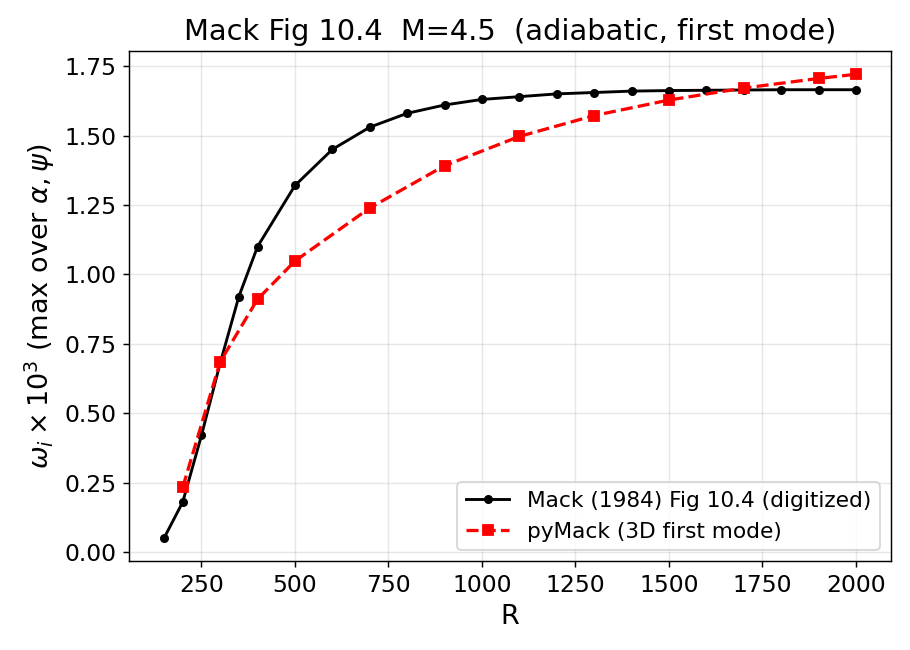
\includegraphics[width=0.75\linewidth]{../verification/first_mode/mack_fig10_4_M45/overlay.png}
\caption{Mack Fig.~10.4 \cite{mack1984}, $M=4.5$: the oblique first mode optimised over
$(\alpha,\psi)$, over the digitised points.}
\label{fig:mack104_m45}
\end{figure}

\begin{figure}[H]
\centering
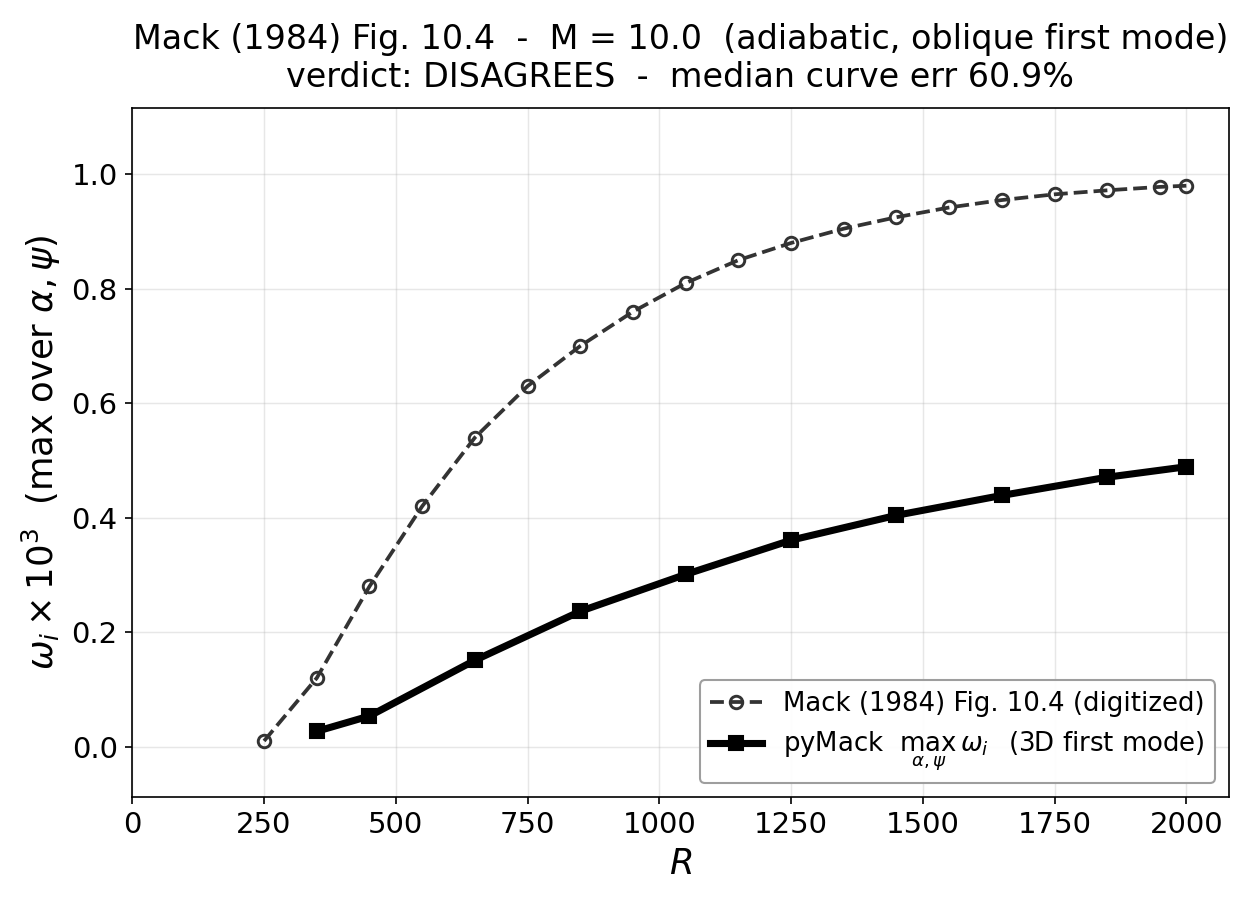
\includegraphics[width=0.75\linewidth]{../verification/first_mode/mack_fig10_4_M100/overlay.png}
\caption{Mack Fig.~10.4 \cite{mack1984}, $M=10$: the same comparison at the top of the Mach range,
with a small residual (lower-confidence magnitude, see text).}
\label{fig:mack104_m100}
\end{figure}

\FloatBarrier
%=====================================================================
\section{Mixed first and second mode: the \"Ozgen--K{\i}rcal{\i} neutral-curve family}
\label{sec:mixedmode}
%=====================================================================
Fig.~3 of \"Ozgen \& K{\i}rcal{\i} \cite{ozgen2008} presents, for each Mach number from 2 to 10, a
single neutral-curve figure in the $(Re_L,\alpha_L)$ plane. At $M=2$ and $3$ the figure contains
the first-mode lobe alone; from $M\approx4$ the second (Mack) mode enters, and each figure then
spans \emph{both} instability families; at $M=6$, for example, four branches: second-mode upper
and lower, first-mode cutoff, and first-mode onset. Because a single reproduced figure tests both
modes at once, these cases are classified neither under the first nor the second mode but as a
mixed family, and they are reported last, drawing on both preceding sections: at $M=2$ and $M=3$
only the first mode is present, while $M=4$--$10$ span both modes.

\paragraph{Reference.} \"Ozgen \& K{\i}rcal{\i} \cite{ozgen2008}, Fig.~3 (M = 2, 3, 4, 6, 7, 8,
10).

\paragraph{Conditions.} Air, adiabatic wall, 2-D ($\psi=0^\circ$); temporal neutral contour
($c_i=0$) in the $(Re_L,\alpha_L)$ plane, with the \"Ozgen temperature-dependent transport laws. The
neutral loci are traced on two Chebyshev grids: the wall-trapped second mode at $N=180$ with
$y_{\max}=8$--$12\,\delta^\ast/L^\ast$, and the more diffuse first mode at $N=200$ with
$y_{\max}=35$--$45\,\delta^\ast/L^\ast$; $L^\ast$ scaling throughout.

The temperature-form 2-D temporal GEVP (the \"Ozgen equation arrangement) is solved over a
$(Re_L,\alpha_L)$ grid, real $\alpha_L$ at each $Re_L$ returning the complex phase speeds. A
discrete-mode extractor (eigenfunction decay $+$ $y_{\max}$-stationarity, the two acceptance tests
of the companion numerical-methods document) selects the physical mode at each node, eigenvalue
continuation carries difficult branches through the grid, and the neutral family (all branches
$\alpha_L(Re_L)$ of both the first and second mode) is the extracted $c_i=0$ contour. This extractor
replaces the earlier $c_r$-band classifier that had excluded the genuine first mode; with that
correction and the references re-digitised, the picture is:
\begin{itemize}[leftmargin=1.4em,itemsep=1pt]
\item \textbf{$M=4$ and $M=6$} (Figures~\ref{fig:ozgen_m4} and \ref{fig:ozgen_m6}): a complete
two-lobe match. At $M=4$ both second-mode branches sit on the digitisation floor and the first-mode
cutoff is reproduced; only the deep low-$\alpha$ onset departs. At $M=6$, after re-digitising the
reference and re-tracing the neutral loci on a grid extended to low $Re$, Our LST code closes both
lobes at their critical Reynolds number (second-mode nose $R\!\approx\!206$ against \"Ozgen's
$\approx\!200$) and reproduces the three robust branches (second-mode upper and lower, first-mode
cutoff); only the first-mode onset runs below the reference, the continuous-spectrum-limited tail.
\item \textbf{$M=2$ and $M=3$} (Figure~\ref{fig:ozgen_m2}): $M=2$ traces both first-mode branches
over the full $R$-range by eigenvalue continuation; at $M=3$ the first-mode cutoff is reproduced
where resolvable, the onset again being continuous-spectrum-blocked.
\item \textbf{$M=7$, $M=8$, $M=10$}: the dominant second-mode cutoff branch is reproduced, but
Our LST code predicts a \emph{connected} first--second-mode band where the reference shows two
lobes separated by a stable gap. This is a connected-vs-separated topology difference (inter-mode
over-prediction at high Mach), not a second-mode-curve error.
\end{itemize}
A separate growth-contour comparison (the $c_i=0.004$ lobe rather than the neutral curve) does not
match, and the interior $c_i=0.012$ M2 lobe is absent because Our LST code's peak M2 growth
$c_{i,\max}=0.0109$ falls just short of $0.012$; this is the same open-lobe / under-amplification
discrepancy noted above. Representative cases for $M=2$, $4$, and $6$ follow
(Figures~\ref{fig:ozgen_m2}, \ref{fig:ozgen_m4}, and \ref{fig:ozgen_m6}); the remaining Mach
numbers ($M=3$, $7$, $8$, and $10$) are summarised in Table~\ref{tab:summary}.

\begin{figure}[H]
\centering
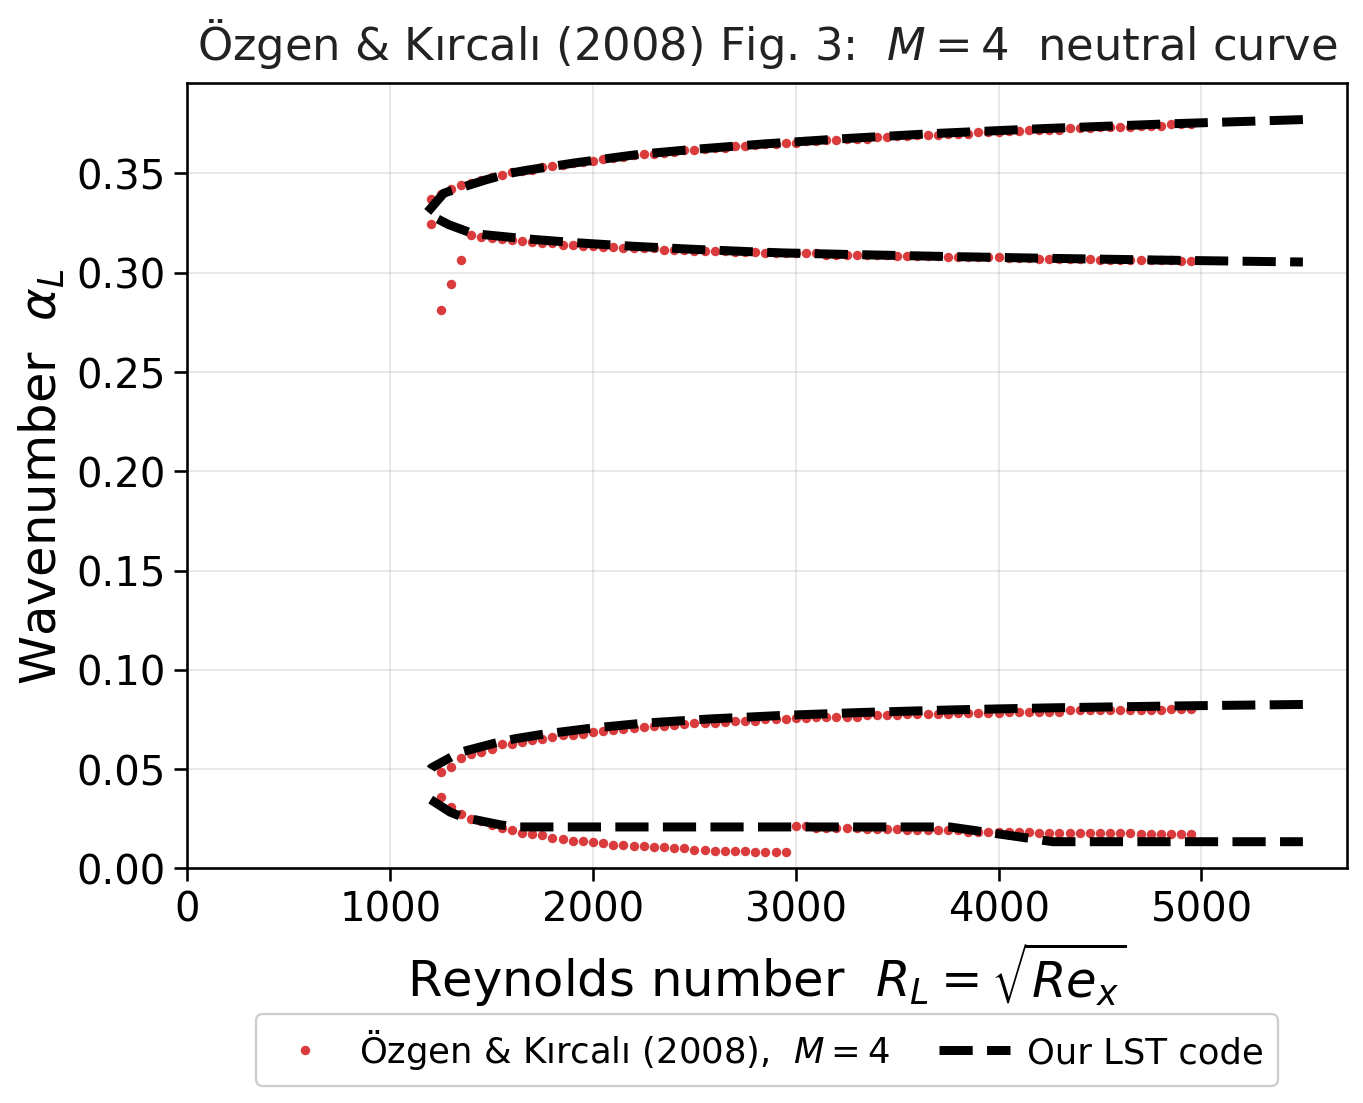
\includegraphics[width=0.95\linewidth]{../verification/mixed_mode/ozgen_fig3/M4/overlay_pub.png}
\caption{\"Ozgen \& K{\i}rcal{\i} Fig.~3 \cite{ozgen2008}, $M=4$: Our LST code reproduces the
entire two-lobe neutral structure, with both second-mode branches on the digitisation floor and the
first-mode cutoff closely tracked.}
\label{fig:ozgen_m4}
\end{figure}

\begin{figure}[H]
\centering
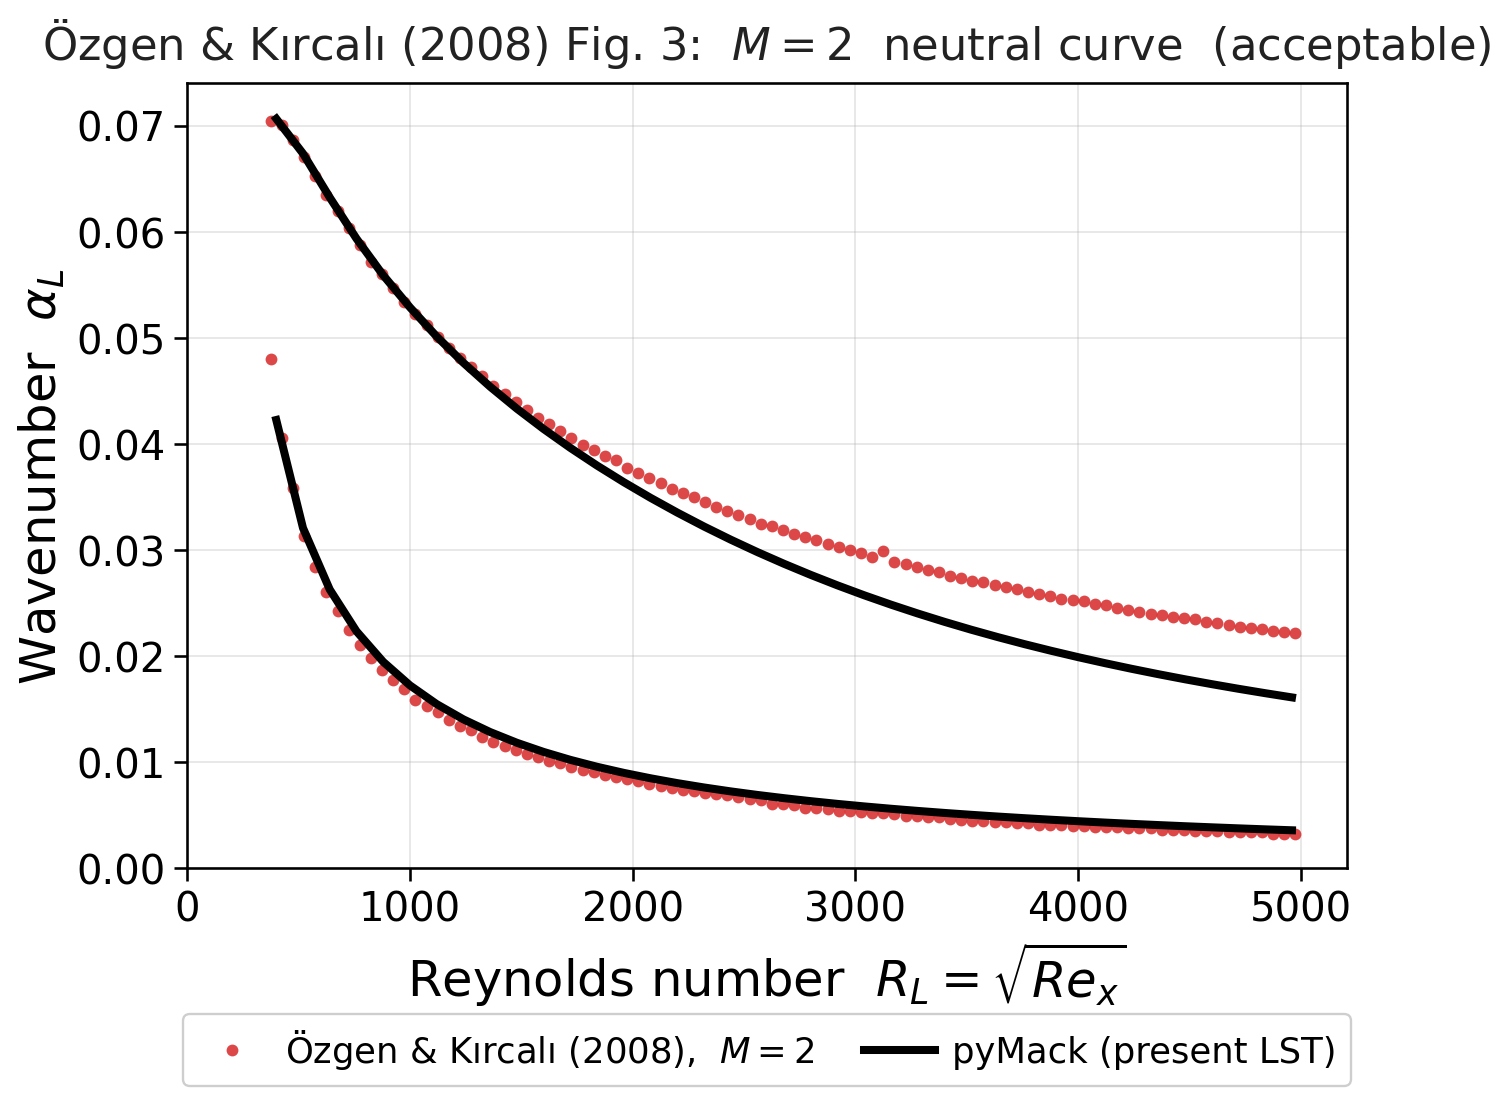
\includegraphics[width=0.95\linewidth]{../verification/mixed_mode/ozgen_fig3/M2/overlay_pub.png}
\caption{\"Ozgen \& K{\i}rcal{\i} Fig.~3 \cite{ozgen2008}, $M=2$ (first mode only at this Mach):
both branches traced over the full $R$-range by eigenvalue continuation.}
\label{fig:ozgen_m2}
\end{figure}

\begin{figure}[H]
\centering
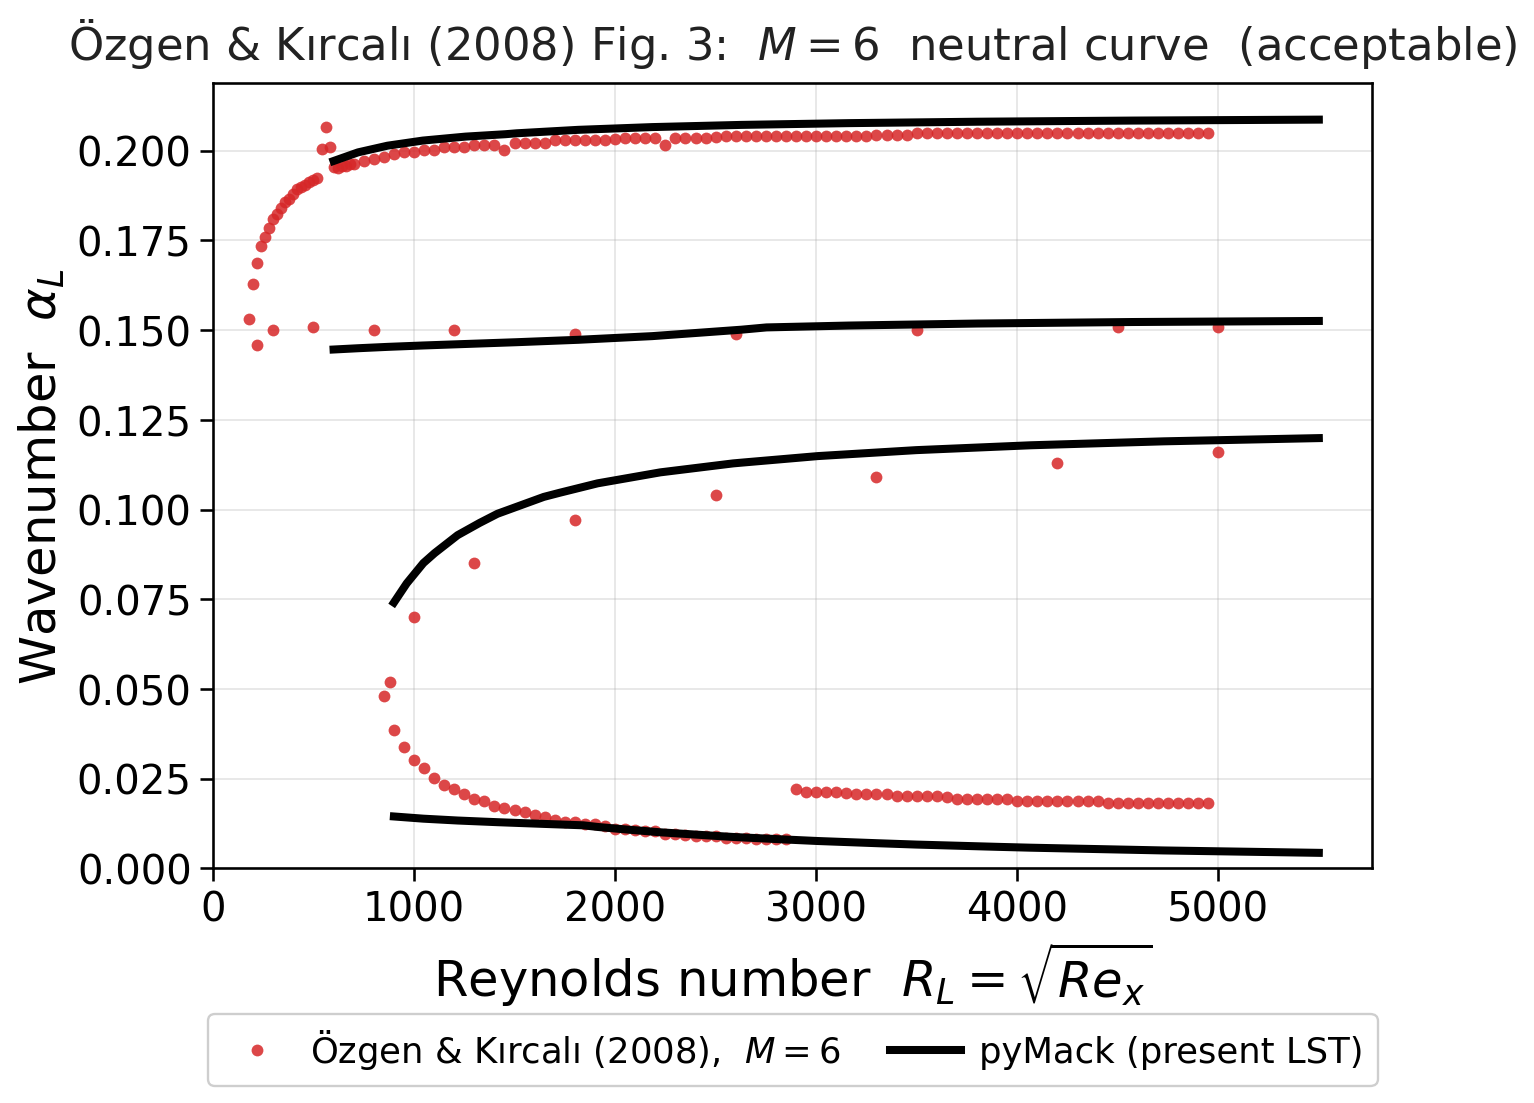
\includegraphics[width=0.95\linewidth]{../verification/mixed_mode/ozgen_fig3/M6/overlay_pub.png}
\caption{\"Ozgen \& K{\i}rcal{\i} Fig.~3 \cite{ozgen2008}, $M=6$ (both modes in one figure): the
re-digitised reference points and Our LST code's full $c_i=0$ contour. Re-tracing the neutral loci
on a grid extended to low $Re$ closes both lobes at their critical Reynolds number, the second-mode
nose sitting at $R\!\approx\!206$ against \"Ozgen's $\approx\!200$. The three robust branches
(second-mode upper and lower, first-mode cutoff) are reproduced; only the deep low-$\alpha$
first-mode onset runs below the reference, the continuous-spectrum-limited tail.}
\label{fig:ozgen_m6}
\end{figure}

\FloatBarrier

\bigskip
\noindent\textit{Cases that are not settled validations (the isolated $M\approx2.2$ first-mode
disagreements, the sharp-cone $N$-factor with its bounded magnitude deficit, the private Mach 5.35
code-to-code benchmark, and the Mach 6 pipeline demonstration) are collected in the companion
working note.}

\begin{thebibliography}{9}
\bibitem{orszag1971} S.~A. Orszag, ``Accurate solution of the Orr--Sommerfeld stability
  equation,'' \emph{Journal of Fluid Mechanics}, Vol.~50, No.~4, 1971, pp.~689--703.
\bibitem{malik1990} M.~R. Malik, ``Numerical methods for hypersonic boundary layer stability,''
  \emph{Journal of Computational Physics}, Vol.~86, No.~2, 1990, pp.~376--413.
\bibitem{balakumar1992} P.~Balakumar and M.~R. Malik, ``Discrete modes and continuous spectra in
  supersonic boundary layers,'' \emph{Journal of Fluid Mechanics}, Vol.~239, 1992, pp.~631--656.
\bibitem{mack1984} L.~M. Mack, ``Boundary-layer linear stability theory,'' AGARD Report No.~709,
  \emph{Special Course on Stability and Transition of Laminar Flow}, 1984.
\bibitem{ozgen2008} S.~\"Ozgen and S.~A. K{\i}rcal{\i}, ``Linear stability analysis in
  compressible, flat-plate boundary layers,'' \emph{Theoretical and Computational Fluid Dynamics},
  Vol.~22, 2008, pp.~1--20.
\bibitem{egorov2006} I.~V. Egorov, A.~V. Fedorov, and V.~G. Soudakov, ``Direct numerical
  simulation of disturbances generated by periodic suction-blowing in a hypersonic boundary
  layer,'' \emph{Theoretical and Computational Fluid Dynamics}, Vol.~20, No.~1, 2006, pp.~41--54.
\bibitem{mazhong2003} X.~Ma and X.~Zhong, ``Receptivity of a supersonic boundary layer over a flat
  plate. Part 1. Wave structures and interactions,'' \emph{Journal of Fluid Mechanics}, Vol.~488,
  2003, pp.~31--78.
\bibitem{xirenfu2020} Xi, Ren, and Fu, arXiv preprint arXiv:2006.05970, 2020.
\bibitem{hildebrand2018} N.~Hildebrand et al., arXiv preprint arXiv:1712.08239, 2017.
\end{thebibliography}

\end{document}
